\documentclass[preprint]{JASAnew}\usepackage[]{graphicx}\usepackage[]{color}
%% maxwidth is the original width if it is less than linewidth
%% otherwise use linewidth (to make sure the graphics do not exceed the margin)
\makeatletter
\def\maxwidth{ %
  \ifdim\Gin@nat@width>\linewidth
    \linewidth
  \else
    \Gin@nat@width
  \fi
}
\makeatother

\definecolor{fgcolor}{rgb}{0.345, 0.345, 0.345}
\newcommand{\hlnum}[1]{\textcolor[rgb]{0.686,0.059,0.569}{#1}}%
\newcommand{\hlstr}[1]{\textcolor[rgb]{0.192,0.494,0.8}{#1}}%
\newcommand{\hlcom}[1]{\textcolor[rgb]{0.678,0.584,0.686}{\textit{#1}}}%
\newcommand{\hlopt}[1]{\textcolor[rgb]{0,0,0}{#1}}%
\newcommand{\hlstd}[1]{\textcolor[rgb]{0.345,0.345,0.345}{#1}}%
\newcommand{\hlkwa}[1]{\textcolor[rgb]{0.161,0.373,0.58}{\textbf{#1}}}%
\newcommand{\hlkwb}[1]{\textcolor[rgb]{0.69,0.353,0.396}{#1}}%
\newcommand{\hlkwc}[1]{\textcolor[rgb]{0.333,0.667,0.333}{#1}}%
\newcommand{\hlkwd}[1]{\textcolor[rgb]{0.737,0.353,0.396}{\textbf{#1}}}%
\let\hlipl\hlkwb

\usepackage{framed}
\makeatletter
\newenvironment{kframe}{%
 \def\at@end@of@kframe{}%
 \ifinner\ifhmode%
  \def\at@end@of@kframe{\end{minipage}}%
  \begin{minipage}{\columnwidth}%
 \fi\fi%
 \def\FrameCommand##1{\hskip\@totalleftmargin \hskip-\fboxsep
 \colorbox{shadecolor}{##1}\hskip-\fboxsep
     % There is no \\@totalrightmargin, so:
     \hskip-\linewidth \hskip-\@totalleftmargin \hskip\columnwidth}%
 \MakeFramed {\advance\hsize-\width
   \@totalleftmargin\z@ \linewidth\hsize
   \@setminipage}}%
 {\par\unskip\endMakeFramed%
 \at@end@of@kframe}
\makeatother

\definecolor{shadecolor}{rgb}{.97, .97, .97}
\definecolor{messagecolor}{rgb}{0, 0, 0}
\definecolor{warningcolor}{rgb}{1, 0, 1}
\definecolor{errorcolor}{rgb}{1, 0, 0}
\newenvironment{knitrout}{}{} % an empty environment to be redefined in TeX

\usepackage{alltt}

\graphicspath{{./graphics/}}

% symbols
\usepackage[utf8]{inputenc}
\usepackage{siunitx}
\usepackage{tipa}
\usepackage{amsmath,mathtools,amssymb}

% URLs
\usepackage{url}

% figure panels
\usepackage{stackengine}

% overbrace on matrices
\newcommand\overmat[2]{%
  \makebox[0pt][l]{$\smash{\color{white}\overbrace{\phantom{%
    \begin{matrix}#2\end{matrix}}}^{\text{\color{black}#1}}}$}#2}
\newcommand\bovermat[2]{%
  \makebox[0pt][l]{$\smash{\overbrace{\phantom{%
    \begin{matrix}#2\end{matrix}}}^{#1}}$}#2}

% participant characteristics table
\usepackage{multirow,array}
\newcommand\Tstrut{\rule{0pt}{2.6ex}}         % = `top' strut
\newcommand\Bstrut{\rule[-0.9ex]{0pt}{0pt}}   % = `bottom' strut
\newcolumntype{L}[1]{>{\raggedright\let\newline\\\arraybackslash\hspace{0pt}}m{#1}}
\newcolumntype{C}[1]{>{\centering\let\newline\\\arraybackslash\hspace{0pt}}m{#1}}
\newcolumntype{R}[1]{>{\raggedleft\let\newline\\\arraybackslash\hspace{0pt}}m{#1}}
\IfFileExists{upquote.sty}{\usepackage{upquote}}{}
\begin{document}



\title[Task dependence of articulator synergies]{Task-dependence of articulator synergies}

\thanks{Portions of this work were presented in 
``Factor analysis of vocal-tract outlines derived from real-time magnetic resonance imaging data,'' International Congress of Phonetic Sciences, Glasgow, UK, 2015,
``Characterizing vocal tract dynamics using real-time MRI,'' LabPhon 2016, Ithaca, NY, 2016,
``Characterizing vocal tract dynamics across speakers using real-time MRI,'' Proceedings of Interspeech, San Francisco, CA, 2016, 
``Decomposing vocal tract constrictions into articulator contributions using real-time MRI,'' Proceedings of the 7th International Conference on Speech Motor Control, Groningen, the Netherlands, 2017,
``Test-retest repeatability of articulatory strategies using real-time magnetic resonance imaging,'' Proceedings of Interspeech 2017, Stockholm, Sweden, 2017.}

\author{Tanner Sorensen}
\affiliation{Signal Analysis and Interpretation Laboratory, Ming Hsieh Department of Electrical Engineering, University of Southern California, Los Angeles, CA 90089, USA}
\affiliation{Department of Linguistics, University of Southern California, Los Angeles, CA 90089, USA}

\author{Asterios Toutios}
\affiliation{Signal Analysis and Interpretation Laboratory, Ming Hsieh Department of Electrical Engineering, University of Southern California, Los Angeles, CA 90089, USA}

\author{Louis Goldstein}
\affiliation{Department of Linguistics, University of Southern California, Los Angeles, CA 90089, USA}

\author{Shrikanth Narayanan}
\affiliation{Signal Analysis and Interpretation Laboratory, Ming Hsieh Department of Electrical Engineering, University of Southern California, Los Angeles, CA 90089, USA}
\affiliation{Department of Linguistics, University of Southern California, Los Angeles, CA 90089, USA}

\begin{abstract}
In speech production, the motor system organizes articulators such as the jaw, tongue, and lips into synergies whose function is to produce speech sounds by forming constrictions at the phonetic places of articulation.
%
The present study tests whether synergies for different constriction tasks differ in terms of inter-articulator coordination.
%
The test is conducted on utterances \textipa{[ApA]}, \textipa{[AtA]}, \textipa{[AiA]}, and \textipa{[AkA]} with a real-time magnetic resonance imaging biomarker that is computed using a statistical model of the forward kinematics of the vocal tract. 
%
The present study is the first to estimate the forward kinematics of the vocal tract from speech production data.
%
Using the imaging biomarker, the study finds that the jaw contributes 
least to the velar stop for \textipa{[k]},
more to pharyngeal approximation for \textipa{[A]}, 
still more to palatal approximation for \textipa{[i]},
and most to the coronal stop for \textipa{[t]}.
%
Additionally, the jaw contributes more to the coronal stop for \textipa{[t]} than to the bilabial stop for \textipa{[p]}.
%
Finally, the study investigates how this pattern of results varies by participant.
%
The study identifies differences in inter-articulator coordination by constriction task that support the claim that inter-articulator coordination differs depending on the active articulator synergy.
\end{abstract}


\maketitle


\section{Introduction}

An articulator synergy is a functional grouping of articulators such as the jaw, tongue, and lips whose coordinated movements produce constrictions during speech, and which instantiates a reduction in the number of independent degrees of freedom for controlling a vocal tract movement~\cite{turvey1977preliminaries}.
%
Phonetic studies have shown that the coordination of articulators differs depending on where in the vocal tract the synergy produces a constriction. 
%
For instance, mechanical perturbations to jaw position during a bilabial stop induce compensatory lip movement with no compensatory tongue movement, 
%
whereas mechanical perturbations to jaw position during a lingual constriction induce compensatory tongue movement with no compensatory lip movement~\citep{kelso1984functionally}. 
%
Our previous study on unperturbed speech suggests that healthy adult speakers of American English may use the jaw more for bilabial stops, coronal stops, and palatal approximations than for velar stops and pharyngeal approximations~\citep{Sorensen+2016}. 
%
Differences in inter-articulator coordination by constriction task support the task-dependence of articulator synergies~\citep{latash2008synergy}. 

The present study investigates the task-dependence of articulator synergies by quantifying the percent contribution of each articulator to narrowing or widening the vocal tract at the synergy's place of articulation. 
%
In the Task Dynamics model of speech production~\citep{saltzman1989dynamical}, the percent contribution of each articulator in a synergy is determined by assigning weights to the articulators. 
%
In contrast to studies that manually assign weights to the articulators based on theoretical considerations~\citep[for example, see][for an assignment of weights based on articulator mass]{simko2010embodied}, the present study is the first to obtain a quantitative readout of these weights from speech production data. 

Advances in magnetic resonance imaging (MRI) have achieved a balance among the competing factors of temporal resolution, spatial resolution, and signal-to-noise ratio that provides a rich source of speech production data for the present study~\citep{scott2014speech}. Real-time MRI pulse sequences and reconstruction techniques allow for the capture and visualization of the motion of the jaw, tongue, and lips with \SI{12}{\milli\second} temporal resolution~\citep{toutios2016advances,lingala2017fast}. 
%
The present study uses real-time MRI to quantify articulator synergies in terms of the percent contribution of each articulator to producing constrictions.
%
The proposed measure of articulator synergies is derived from in vivo MRI as a descriptor of articulator synergies (i.e., a quantitative imaging biomarker, ``an objective characteristic derived from an in vivo image measured on a ratio or interval scale as an indicator of normal biological processes'', \citealt{kessler2015emerging,sullivan2015metrology}). 





The algorithm for computing the articulator synergy biomarker involves a statistical model of the forward kinematics of the vocal tract. The forward kinematics relates articulator parameters to constriction task variables, as in the Task Dynamics model of speech production (\citealt{saltzman1989dynamical}; see \citealt{lammert2013statistical} for a procedure of estimating the forward kinematics of the vocal tract from synthetic data). 
%
The forward kinematics has two parts: the direct and differential kinematics.
%
The direct kinematics expresses the degree of constriction (i.e., constriction task variable, measured in millimeters) at the phonetic places of articulation as a function of the position and shape of articulators. 
%
This function is called the forward kinematic map. 
%
The differential kinematics expresses change in the constriction task variables as a function of small increments of articulator movement.
%
This function is the jacobian matrix of the forward kinematic map. 
%
The algorithm uses the jacobian matrix of the forward kinematic map to compute the percent contribution of each articulator to narrowing or widening the vocal tract at the synergy's place of articulation. 






The research goals of the present study are 
%
(i) to estimate and evaluate the forward kinematics of the vocal tract from MRI, 
%
(ii) to design and evaluate a biomarker of articulator synergies based on the forward kinematics, and
%
(iii) to use the articulator synergy biomarker to test the task-dependence of articulator synergies by determining whether the relative contribution of the jaw, tongue, and lips differs by constriction task. 


The paper is organized as follows.
%
Section~\ref{sec:mri} describes the MRI experiment, scanner sequence, participant characteristics, and method for manually annotating the start and end time-points in the real-time MRI videos. 
Sections~\ref{sec:cd} and~\ref{sec:gfa} describe the segmentation of articulator contours in the images and use the segmentation results to estimate constriction task variables and parameters of articulator shape and position, which are related by the forward kinematics of the vocal tract. 
Section~\ref{sec:forwardkinematicmap} estimates the forward kinematics and evaluates the model through cross-validation. 
Section~\ref{sec:articulator_synergy_biomarker} defines the articulator synergy biomarker. It evaluates the articulator synergy biomarker with respect to bias and precision. 
Section~\ref{sec:taskspec} tests the effect of constriction task on the articulator synergy biomarker. Confirming this effect shows that inter-articulator coordination differs by constriction task, supporting the task-specificity of articulator synergies. 
Section~\ref{sec:patterns} investigates differences by participant in the effect of constriction task on the articulator synergy biomarker as well as intra-participant variability in biomarker values.
Sections~\ref{sec:discussion} and~\ref{sec:conclusions} offer discussion and conclusions.



\section{Magnetic resonance imaging}
\label{sec:mri}

\subsection{Experiment}
\label{subsec:experimentdescription}

The data-set included eight (4 male, 4 female) speakers of American English~\cite{toger2017test}. Five participants were native speakers of American English. None of the participants reported speech pathology or abnormal hearing. Table~\ref{tab:subj2} provides participant characteristics. Each participant took part in one session. The authors explained the nature of the experiment and the protocol to the participant before each scan. The participant lay on the scanner table in a supine position. The head was fixed in place by foam pads inserted between the temple and the receiver coil on the left and right sides of the head. The participant read visually presented text from a paper card taped to the scanner bore in front of the face. The speech corpus included real-time MRI videos of the isolated utterances \textipa{[ApA]}, \textipa{[AtA]}, \textipa{[AkA]}, and \textipa{[AiA]} produced in an unrandomized sequence. Although participants were instructed to produce a low back unrounded vowel \textipa{[A]} and high front unrounded vowel \textipa{[i]}, there was some variability in whether the low vowel was the front \textipa{[a]} or back \textipa{[A]} and in whether or not the high vowel was produced as a glide \textipa{[j]}. Participants produced the sequence of utterances ten times. The authors removed the participant from the scanner for a short break, and then repeated the experiment. After completing the session, the speaker was paid for their participation in the study. The USC Institutional Review Board approved the data collection procedures. 

\begin{table}
\centering
\begin{tabular}{l l l L{0.2\linewidth} l}
\hline
ID & age & gender & state of origin & native language \Tstrut \Bstrut \\
\hline
F1 & 25 & F & Rhode Island & American English \Tstrut \\
F2 & 28 & F & Texas & American English \\
F3 & 24 & F & Nebraska & American English \\
F4 & 29 & F & Korea & Korean \\
M1 & 29 & M & Iowa & American English \\
M2 & 27 & M & United Arab Emirates & American English \\
M3 & 26 & M & Germany & German \\
M4 & 39 & M & Greece & Greek \\
\hline
& \shortstack[l]{\Tstrut median: 28 \\ range: 24--39}
& \shortstack[l]{\Tstrut 4 male \\ 4 female}
&
& \shortstack[l]{5 American English \\ 3 other}\Tstrut \Bstrut \\
\hline
\end{tabular}
\caption{Participant characteristics of the test-retest data-set}
\label{tab:subj2}
\end{table}

Vocal tract constrictions were manually identified in the real-time MRI videos. 
%
The video frames were inspected on a computer monitor. 
%
Guided by graphical presentation of real-time MRI video frames and auditory presentation of a denoised speech audio signal recorded in the scanner bore, the authors manually identified the intervals of time during which the vocal tract produced the bilabial stop in \textipa{[ApA]}, coronal stop in \textipa{[AtA]}, palatal approximation in \textipa{[AiA]}, velar stop in \textipa{[AkA]}, and pharyngeal approximation in \textipa{[AiA]} (second \textipa{[A]} used for pharyngeal approximation). 
%
The authors annotated the frame number of the first and last frames in which there was visible movement of the lips (for \textipa{[ApA]}) or tongue (for \textipa{[AtA]}, \textipa{[AkA]}, and \textipa{[AiA]}). 




\subsection{Imaging parameters}

Data were acquired on a Signa Excite HD \SI{1.5}{\tesla} scanner (General Electric Healthcare, Waukesha WI) with gradients capable of \SI[per-mode=symbol]{40}{\milli\tesla\per\meter} amplitude and \SI[per-mode=repeated-symbol]{150}{\milli\tesla\per\meter\per\milli\second} slew rate. A custom eight-channel upper airway coil was used for radio frequency signal reception. The coil had two 4-channel arrays. 
%
A real-time MRI pulse sequence based on a spiral fast gradient echo pulse sequence was used. 
%
The real-time MRI pulse sequence parameters were the following: 
%
\SI{200 x 200}{\milli\meter} field of view, 
\SI{2.4 x 2.4}{\milli\meter} reconstructed in-plane spatial resolution, 
\SI{6}{\milli\meter} slice thickness,
\SI{6}{\milli\second} TR,
\SI{3.6}{\milli\second} TE,
\SI{15}{\degree} flip angle,
\num{13} spiral interleaves for full sampling.
%
The scan plane was manually aligned to the head. 
%
Images were retrospectively reconstructed to a temporal resolution of \SI{12}{\milli\second} (\SI{6}{\milli\second} TR times two spirals per image, 83 frames per second). 
%
Reconstruction was performed using the Berkeley Advanced Reconstruction Toolbox~\cite{uecker2015berkeley}.







\section{Constriction task variable measurement}
\label{sec:cd}

The contours of articulators were identified in the real-time MRI videos and tracked automatically during vocal tract constrictions~\citep{bresch2009region}. The algorithm was manually initialized with templates matching vocal tract contours during the sounds \textipa{[A], [i], [p], [t], [k]} (Fig.~\ref{fig:segtemp}). 
%
If visual inspection revealed clear errors, then the algorithm initialization was manually corrected and the contours were re-submitted to the algorithm. This was repeated as needed until no clear contour tracking errors remained. 
%
See Fig.~\ref{fig:segtemp} for example segmentation results.

\begin{figure}

\includegraphics[width=\linewidth]{SegTempFigure.pdf}

\caption{(color online) {\bf a.} Subject-specific templates for \textipa{[A]}, \textipa{[i]}, \textipa{[p]}, \textipa{[t]}, \textipa{[k]}, which are automatically deformed to fit the articulator contours in the real-time magnetic resonance images.
{\bf b.} Articulator contour segmentation of a sequence of real-time magnetic resonance images acquired in the transition from \textipa{[A]} to \textipa{[i]} in \textipa{[AiA]}. Frame rate downsampled for presentation.}
\label{fig:segtemp}
\end{figure}



An algorithm automatically measured constriction task variables at the phonetic places of articulation in each video frame. 
%
As we use the term in this study, a constriction task variable is defined as the shortest distance between opposing structures at a given place of articulation. 
%
The opposing structures were the upper and lower lips for \textipa{[p]} (bilabial constriction task variable), tongue and coronal place for \textipa{[t]} (coronal constriction task variable), tongue and palatal place for \textipa{[i]} (palatal constriction task variable), tongue and soft palate for \textipa{[k]} (velar constriction task variable), and tongue and rear pharyngeal wall for \textipa{[A]} (pharyngeal constriction task variable). 
%
The contour tracking algorithm automatically identified the upper lip, lower lip, tongue, hard palate, soft palate, and rear pharyngeal wall~\citep{bresch2009region}.  
%
The anterior \num{1/4} of the hard palate was the coronal place of articulation. 
%
The posterior \num{1/2} of the hard palate was the palatal place of articulation.
%
The velar place was bounded anteriorly by the anterior edge of the soft palate and extended posteriorly over \num{1/8} of the total soft palate contour, which included the oral, uvular, oropharyngeal, and nasal surfaces of the soft palate (cf. gray soft palate contours in~\ref{fig:segtemp}).
%
The pharyngeal place was the posterior pharyngeal wall, bounded superiorly by the velopharyngeal port and inferiorly by the larynx. 
%
Fig.~\ref{fig:constrictions} illustrates the constriction task variable measurements at the phonetic places of articulation.


\begin{figure}

\includegraphics[width=\linewidth]{ConstrictionsFigure.pdf}

\caption{(color online) Constriction task variable at the phonetic places of articulation in the transition from \textipa{[A]} to \textipa{[i]} in the sequence \textipa{[AiA]}. The phonetic places of articulation (blue lines) are bilabial place, coronal place, palatal place, velar place, and pharyngeal place. Frame rate downsampled for presentation.}
\label{fig:constrictions}
\end{figure}




\section{Guided factor analysis of vocal tract shapes}
\label{sec:gfa}




\subsection{Objective of the guided factor analysis}
\label{subsec:objectivesoftheguidedfactoranalysis}

The guided factor analysis of the present study is based on the approach of~\citet{toutios2015factor} and motivated by the analysis of~\citet{maeda1990compensatory}, which extracts factors of the jaw, tongue, and lip articulators (\citeauthor{maeda1990compensatory}’s ``elementary articulators’’) and factor scores that parameterize how the position and shape of these articulators change over time (\citeauthor{maeda1990compensatory}’s ``elementary gestures’’). In this framework, vocal tract movements are the sum of a few elementary gestures, which are factors in our analysis. 

The objective of the guided factor analysis was to parameterize the vocal tract contours $\mathbf{X} \in \mathbb{R}^{n\times 2p}$, where $n$ is the number of images and $p$ is the number of contour vertices, as the linear combination of factors $\mathbf{f}_1, \mathbf{f}_2, \ldots, \mathbf{f}_q \in \mathbb{R}^{2p}$ such that each factor characterizes spatial variation in the position and shape of an articulator (specifically, the jaw, tongue, lips, and velum). 
%
Prior to the factor analysis, the vocal tract contours $\mathbf{X}$ were centered on zero.
%
The time-varying coefficients $\mathbf{w}_{\cdot,1},\mathbf{w}_{\cdot,2},\ldots,\mathbf{w}_{\cdot,p} \in \mathbb{R}^n$ of the linear combination are factor scores that characterize temporal variation in the position and shapes of the articulators. Factor scores change from one image to the next as the articulators move and change shape. Thus, changes in the factor scores parameterize articulator motion.
%
The guided factor analysis is based on the approach of~\citet{toutios2015factor}.


Factors $\mathbf{f}_1, \mathbf{f}_2, \ldots, \mathbf{f}_q \in \mathbb{R}^{2p}$ are the columns of the matrix $\mathbf{F} \in \mathbb{R}^{2p\times q}$. 
%
Rows $\mathbf{w}_{1,\cdot},\mathbf{w}_{2,\cdot},\ldots,\mathbf{w}_{n,\cdot}$ of the matrix $\mathbf{W} \in \mathbb{R}^{n\times q}$ contain the factor scores for images $1,2,\ldots,n$ of the real-time MRI data-set. 
%
Thus, the contour vertices $\mathbf{x}_{i,\cdot}$ for the $i$th image of the real-time MRI data-set are approximately equal to the following linear combination of the factors. 
%
\begin{align}
\label{eq:linearcombo}
\mathbf{\hat{x}}_{i,\cdot}
 &=
  \mathbf{w}_{i,\cdot} \mathbf{F}^\intercal \\
 &=
  w_{i,1} \mathbf{f}_{\cdot,1}^\intercal
  + w_{i,2} \mathbf{f}_{\cdot,2}^\intercal
  + \ldots
  + w_{i,q} \mathbf{f}_{\cdot,q}^\intercal
\end{align}




The motion of the tongue and lips systematically co-occurs with motion of the jaw due to mechanical constraints and regularities in motor commands. For this reason, we seek a factor that corresponds to the motion of the jaw along with the concomitant motion of the tongue and lips.


The set of $q_\text{jaw}$ jaw factors $\mathbf{F}_\text{jaw} \in \mathbb{R}^{2p\times q_\text{jaw}}$ parameterizes motion of the jaw along with concomitant motion of the tongue, lips, and velum.
%
The set of $q_\text{tongue}$ tongue factors $\mathbf{F}_\text{tongue} \in \mathbb{R}^{2p\times q_\text{tongue}}$ parameterizes motion of the tongue that is independent of the jaw. 
%
The set of $q_\text{lips}$ lip factors $\mathbf{F}_\text{lips} \in \mathbb{R}^{2p\times q_\text{lips}}$ parameterizes motion of the lips that is independent of the jaw.
%
The set of $q_\text{velum}$ velum factors $\mathbf{F}_\text{velum} \in \mathbb{R}^{2p\times q_\text{velum}}$ parameterizes motion of the velum.
%
The full set of factors can be written as the block matrix $\mathbf{F} \in \mathbb{R}^{2p\times q}$, where $q=q_\text{jaw}+q_\text{tongue}+q_\text{lips}+q_\text{velum}$. 
% 
\begin{equation}
\label{eq:Fblock}
\mathbf{F} = 
\left[
\begin{array}{c|c|c|c}
\mathbf{F}_\text{jaw} 
& \mathbf{F}_\text{tongue}
& \mathbf{F}_\text{lips}
& \mathbf{F}_\text{velum}
\end{array}
\right]
\end{equation}
%
The corresponding set of factor scores can be written as the block matrix $\mathbf{W} \in \mathbb{R}^{n\times q}$, where $n$ is the number of MR images in the data-set and $q=q_\text{jaw}+q_\text{tongue}+q_\text{lips}+q_\text{velum}$. 
% 
\begin{equation}
\label{eq:Wblock}
\mathbf{W} = 
\left[
\begin{array}{c|c|c|c}
\mathbf{W}_\text{jaw} 
& \mathbf{W}_\text{tongue}
& \mathbf{W}_\text{lips}
& \mathbf{W}_\text{velum}
\end{array}
\right]
\end{equation}

Section~\ref{subsec:preliminaries} is a preliminary technical note. Section~\ref{subsec:jawfactors} derives the jaw factors. Section~\ref{subsec:residfactors} derives the tongue, lip, and velum factors. Section~\ref{subsec:weights} derives the factor scores. 





\subsection{Preliminaries to the guided factor analysis}
\label{subsec:preliminaries}

Different steps of the guided factor analysis focus on different articulators.
%
The guided factor analysis uses a projection operator to set to zero the contour vertices of articulators not under analysis in a given step of the analysis.
% 
For example, in order to derive the matrix $\mathbf{X}_\text{jaw} \in \mathbb{R}^{n\times 2p}$ that contains only jaw contour vertices, the guided factor analysis sets to zero the contour vertices (i.e., columns of $\mathbf{X}$) of all non-jaw articulators and leaves the contour vertices of the jaw unchanged. 
%
Specifically, the non-jaw contour vertices are set to zero by multiplying $\mathbf{X}$  
% 
by the diagonal projection matrix $\mathbf{P}_\text{jaw} \in \mathbb{R}^{2p\times 2p}$. 
% 
We have that $p_{i,i}=1$ if the $i$th column of $\mathbf{X}$ is a jaw vertex. Otherwise, $p_{i,i}=0$. 
% 
This projection operator sets to zero the columns of $\mathbf{X}$ corresponding to non-jaw contour vertices. 
% 
If jaw contour vertices are in columns $q_1,q_2,\ldots,q_\ell$ of $\mathbf{X}$, then the projection works out to the following. 
% 
\begin{equation}
\begin{split}
  \mathbf{X}_\text{jaw} &= \mathbf{X} \mathbf{P}_\text{jaw} \\[10pt]
%
  \left[ {\begin{array}{ccccc}
   0 & \bovermat{\text{jaw contour vertices}}{x_{1,q_1} &  \cdots & x_{1,q_\ell}} & 0 \\
   0 & x_{2,q_1} &  \cdots & x_{2,q_\ell} & 0 \\
   \vdots & \vdots & & \vdots & \vdots \\
   0 & x_{n,q_1} & \cdots & x_{m,q_\ell} & 0 \\
  \end{array} } \right]
%
  &= 
%
   \mathbf{X}
%
   \left[ {\begin{array}{ccccc}
   \bovermat{\text{columns } q_1,\ldots,q_\ell}{0&&&&}\\
   & 1 &&&\\
   && \ddots &&\\
   &&& 1 &\\
   &&&& 0 \\
  \end{array} } \right]
\end{split}
\end{equation}
%
Similarly, the matrices $\mathbf{X}_\text{tongue},\mathbf{X}_\text{lips},\mathbf{X}_\text{velum} \in \mathbb{R}^{n\times 2p}$ focus on the tongue and lip contours, respectively. 
% 
Summing such matrices produces a matrix that corresponds to a set of articulators. For instance, the matrix $\mathbf{X}_{\text{jaw,tongue,lips}} = \mathbf{X}_\text{jaw} + \mathbf{X}_\text{tongue} + \mathbf{X}_\text{lips}$ corresponds to the jaw, tongue, and lips.





\subsection{Jaw factors}
\label{subsec:jawfactors}

We first obtained the factors $\mathbf{F}_\text{jaw}$ that capture the contribution of the jaw to vocal tract shaping (see the jaw factor in Fig.~\ref{fig:gfa}). 
% 
We performed principal component analysis of the jaw (i.e., mandible and chin, cf. Fig.~\ref{fig:segtemp}) contour vertices through eigendecomposition of the covariance matrix $\boldsymbol{\Sigma}_\text{jaw} = \mathbf{X}_\text{jaw}^\intercal \mathbf{X}_\text{jaw}/(n-1)$ into an orthogonal matrix $\mathbf{Q}_\text{jaw} \in \mathbb{R}^{2p\times q_\text{jaw}}$ whose columns are the principal axes of $\mathbf{X}_\text{jaw}$ and a diagonal matrix $\boldsymbol{\Lambda}_\text{jaw} \in \mathbb{R}^{q_\text{jaw} \times q_\text{jaw}}$ whose diagonal entries are the variances of $\mathbf{X}_\text{jaw}$ on the principal axes.
% 
\begin{equation}
\boldsymbol{\Sigma}_\text{jaw} = \mathbf{Q}_\text{jaw}\boldsymbol{\Lambda}_\text{jaw} \mathbf{Q}_\text{jaw}^{-1}
\end{equation}
%
The principal axes $(\mathbf{q}_\text{jaw})_{\cdot,1}$, $(\mathbf{q}_\text{jaw})_{\cdot,2}$, $\ldots$, $(\mathbf{q}_\text{jaw})_{\cdot,q_\text{jaw}}$ and the variances $(\lambda_\text{jaw})_{1,1}$, $(\lambda_\text{jaw})_{2,2}$, $\ldots$, $(\lambda_\text{jaw})_{q_\text{jaw},q_\text{jaw}}$ on these axes capture the direction and variance of jaw motion. 
% 
The jaw factors $(\mathbf{f}_\text{jaw})_{\cdot,1}$, $(\mathbf{f}_\text{jaw})_{\cdot,2}$, $\ldots$, $(\mathbf{f}_\text{jaw})_{\cdot,q_\text{jaw}}$ capture this jaw motion along with concomitant tongue and lip motion.
% 
The jaw factors are the columns of matrix $\mathbf{F}_\text{jaw} \in \mathbb{R}^{2p\times q_\text{jaw}}$. 
%
\begin{equation}
\mathbf{F}_\text{jaw}
 = \boldsymbol{\Sigma}_\text{jaw,tongue,lips} \mathbf{Q}_\text{jaw} \boldsymbol{\Lambda}_\text{jaw}^{-1/2}
\end{equation}
%
Column $(\mathbf{f}_\text{jaw})_{\cdot,i}$ is the vector of covariances between the jaw, tongue, and lip contour vertices and the z-scored component scores $\mathbf{X} (\mathbf{q}_\text{jaw})_{\cdot,i} / \sqrt{(\lambda_\text{jaw})_{i,i}}$ for the $i$th jaw principal component. 
%
Thus, the factors capture motion of the tongue and lips which accompanies the motion of the jaw. 
%
Note that the matrix $\boldsymbol{\Lambda}_\text{jaw}^{-1/2}$ is the inverse of the principal square root of $\boldsymbol{\Lambda}_\text{jaw}$.
%
Postmultiplying $\boldsymbol{\Sigma}_\text{jaw,tongue,lips} \mathbf{Q}_\text{jaw}$ by $\boldsymbol{\Lambda}_\text{jaw}^{-1/2}$ z-scores the component scores $\mathbf{X}\mathbf{Q}_\text{jaw}$, whose covariances with the jaw, tongue, and lip contour vertices $\mathbf{X}_\text{jaw,tongue,lips}$ are the entries of the jaw factors $\mathbf{F}_\text{jaw}$.

The column space $\mathrm{Col}(\mathbf{F}_\text{jaw})$ of $\mathbf{F}_\text{jaw}$ is a $q_\text{jaw}$-dimensional subspace of $\mathbb{R}^{2p}$. 
%
Variance within $\mathrm{Col}(\mathbf{F}_\text{jaw})$ captures jaw contour motion and concomitant tongue and lip motion (see Fig.~\ref{fig:varexpl}, panel a).
%
The projection $\mathbf{\hat{X}}$ of the data $\mathbf{X}$ on the space $\mathrm{Col}(\mathbf{F}_\text{jaw})$ is obtained through the Moore-Penrose pseudoinverse $\mathbf{F}_\text{jaw}^+$ of $\mathbf{F}_\text{jaw}$. 
%
\begin{equation} \label{eq:XXuu}
\mathbf{\hat{X}} 
= \mathbf{X} 
  \mathbf{F}_\text{jaw}
  \mathbf{F}_\text{jaw}^+ 
\end{equation}
%
The null space $\mathrm{Null}(\mathbf{F}_\text{jaw}^\intercal)$ is a $(p-q_\text{jaw})$-dimensional subspace of $\mathbb{R}^{2p}$. 
% 
Variance within $\mathrm{Null}(\mathbf{F}_\text{jaw}^\intercal)$ captures velum motion along with the part of tongue and lip motion that is independent of jaw motion. 
%
Section~\ref{subsec:residfactors} describes the factors that characterize the variance of the tongue, lips, and velum within $\mathrm{Null} \left( \mathbf{F}_\text{jaw}^\intercal \right)$. 





\subsection{Tongue, lip, and velum factors}
\label{subsec:residfactors}

This section describes the procedure for obtaining the factors $\mathbf{F}_\text{tongue}$ that capture the contribution of the tongue to vocal tract shaping  (see the tongue factors in Fig.~\ref{fig:gfa}). 
% 
The projection $\mathbf{\tilde{X}}$ of the data matrix $\mathbf{X}$ on the space $\mathrm{Null}(\mathbf{F}_\text{jaw}^\intercal)$ is the contour vertex motion that is independent of the jaw.
%
\begin{align} \label{eq:XXX}
\mathbf{\tilde{X}} 
&= \mathbf{X} \left( \mathbf{I}_p - \mathbf{F}_\text{jaw}\mathbf{F}_\text{jaw}^+ \right) \\
&= \mathbf{X} - \mathbf{\hat{X}} 
\end{align}
%
Specifically, $\mathbf{\tilde{X}}$ is independent of the jaw in the sense that it is statistically independent of $\mathbf{\hat{X}}$. 
%
% Appendix~\ref{sec:independence} provides a proof of independence.  





We performed principal component analysis of the tongue contour vertices through eigendecomposition of the covariance matrix $\boldsymbol{\tilde{\Sigma}}_\text{tongue} = \mathbf{\tilde{X}}_\text{tongue}^\intercal \mathbf{\tilde{X}}_\text{tongue}/(n-1)$ into an orthogonal matrix $\mathbf{Q}_\text{tongue}$ whose columns are the principal axes of $\mathbf{\tilde{X}}_\text{tongue}$ and a diagonal matrix $\boldsymbol{\Lambda}_\text{tongue}$ whose diagonal entries are the variances of $\mathbf{\tilde{X}}_\text{tongue}$ on the principal axes.
% 
\begin{equation}
\boldsymbol{\tilde{\Sigma}}_\text{tongue} = \mathbf{Q}_\text{tongue} \boldsymbol{\Lambda}_\text{tongue} \mathbf{Q}_\text{tongue}^{-1}
\end{equation}
%
The principal axes $(\mathbf{q}_\text{tongue})_{\cdot,1}$, $(\mathbf{q}_\text{tongue})_{\cdot,2}, \ldots$, $(\mathbf{q}_\text{tongue})_{\cdot,q_\text{tongue}}$ and the variances $(\lambda_\text{tongue})_{1,1}$, $(\lambda_\text{tongue})_{2,2}, \ldots$, $(\lambda_\text{tongue})_{q_\text{tongue},q_\text{tongue}}$ on these axes capture the direction and variance of tongue motion.


Column $(\mathbf{f}_\text{tongue})_{\cdot,i}$ of the tongue factor matrix $\mathbf{F}_\text{tongue}$ is the vector of covariances between the tongue contour vertices and the z-scored component scores $\mathbf{X} (\mathbf{q}_\text{tongue})_{\cdot,i} / \sqrt{(\lambda_\text{tongue})_{i,i}}$ for the $i$th tongue principal component. 
%
\begin{equation}
\mathbf{F}_\text{tongue}
 = \boldsymbol{\tilde{\Sigma}}_\text{tongue} \mathbf{Q}_\text{tongue} \boldsymbol{\Lambda}_\text{tongue}^{-1/2}
\end{equation}


The column space $\mathrm{Col}(\mathbf{F}_\text{tongue})$ of $\mathbf{F}_\text{tongue}$ is a $q_\text{tongue}$-dimensional subspace of $\mathbb{R}^{2p}$. 
%
Variance within $\mathrm{Col}(\mathbf{F}_\text{tongue})$ captures tongue contour motion that is not concomitant with jaw motion (see Fig.~\ref{fig:varexpl}, panels b and c). 
%
The procedure for deriving lip and velum factors is the same as for the tongue factors except that $\mathbf{X}_\text{lips}$ or $\mathbf{X}_\text{velum}$ is substituted for $\mathbf{X}_\text{tongue}$.




\subsection{Factor scores}
\label{subsec:weights}

According to Equation~\ref{eq:linearcombo}, the data matrix $\mathbf{X}$ is parameterized as the matrix product $\mathbf{W}\mathbf{F}^\intercal$. 
%
Sections~\ref{subsec:jawfactors} and~\ref{subsec:residfactors} specify the factors $\mathbf{F}$. 
%
This section derives the factor scores $\mathbf{W}$ from the factors $\mathbf{F}$ and the data matrix $\mathbf{X}$. 
%
\begin{equation}
\mathbf{W} 
 = \mathbf{X} \left( \mathbf{F}^\intercal \right) ^+
\end{equation}
%
Superscript ``+'' denotes the Moore-Penrose pseudoinverse.
%
In image $i$ of the real-time MRI data-set, the vocal tract contours $\mathbf{x}_{i,\cdot}$ is approximately equal to the linear combination $w_{i,1} \mathbf{f}_1^\intercal + w_{i,2} \mathbf{f}_2^\intercal + \ldots + w_{i,q} \mathbf{f}_q^\intercal$. The factor scores $w_{i,\cdot }$ are the coefficients of the linear combination. Variance of the factor scores parameterizes the temporal variability of vocal tract shape. 

\begin{figure}

\includegraphics[width=0.99\linewidth]{FactorsFigure.pdf}

\caption{(color online) Factors obtained for one participant with one jaw factor, four tongue factors, two lip factors, and one velum factor ($q_\text{jaw} = 1$, $q_\text{tongue} = 4$, $q_\text{lip} = 2$, $q_\text{velum} = 1$). 
Each factor characterizes spatial variation in the position and shape of an articulator. 
The jaw factor captures jaw contour motion and concomitant tongue and lip motion.
The tongue, lip, and velum factors capture tongue and lip contour motion that is not concomitant with jaw motion. 
The articulator contours in a given real-time magnetic resonance image are parameterized as the linear combinations of the factors. 
For a given participant, the coefficients of this linear combination change from image to image as the articulators move, while the factors remain constant.}
\label{fig:gfa}
\end{figure}

\begin{figure*}

\includegraphics[width=0.99\linewidth]{VarExplFigure.pdf}

\caption{(color online) Percent variance explained {\bf (a)} for the mandible and chin contours for each number of jaw factors, {\bf (b)} for the tongue contour for different numbers of jaw and tongue factors, and {\bf (c)} for the lip contours for different numbers of jaw and lip factors. Results averaged over participants.}
\label{fig:varexpl}
\end{figure*}






\section{Forward kinematic map of the vocal tract}
\label{sec:forwardkinematicmap}

\subsection{Estimation of the direct and differential kinematics}

The forward kinematic map is the function that maps the shape and position of the articulators (here parameterized by factor scores) to the corresponding constriction task variables at the phonetic places of articulation~\citep{lammert2013statistical}. 
%
Although the function is nonlinear, in the neighborhood of a given point $\mathbf{w}_{j,\cdot}$ the function can be linearized to have the form of a linear system of equations.
%
Specifically, the linearized forward kinematic map is the function $\mathbf{G}$, where $\mathbf{w} \in \mathbb{R}^q$ is a vector of $q$ factor scores and $\mathbf{z} \in \mathbb{R}^{m}$ is a vector of constriction task variables at the $m$ phonetic places of articulation. 
%
\begin{align}
\mathbf{z} 
&= 
\mathbf{G}\left( \mathbf{w} \right) 
\left[ \begin{array}{c} 1 \\ \mathbf{w} \end{array} \right] \\
&= 
\left[ \begin{array}{cc} 
\boldsymbol{\mu}\left(\mathbf{w}\right) & \mathbf{J}\left(\mathbf{w}\right) 
\end{array} \right]
\left[ \begin{array}{c} 1 \\ \mathbf{w} \end{array} \right]
\end{align}
%
The first column $\mathbf{g}_{\cdot,1}(\mathbf{w})$ of the matrix $\mathbf{G}(\mathbf{w}) \in \mathbb{R}^{m\times (q+1)}$ is the vector $\boldsymbol{\mu}(\mathbf{w}) \in \mathbb{R}^m$ of intercepts for each constriction task variable in the neighborhood of $\mathbf{w}$. 
%
The remaining columns $\mathbf{g}_{\cdot,2}(\mathbf{w}), \ldots, \mathbf{g}_{\cdot,q+1}(\mathbf{w})$ define the jacobian $\mathbf{J}(\mathbf{w})$ of the forward kinematic map in the neighborhood of $\mathbf{w}$. 
% 
\begin{align}
\mathbf{J}(\mathbf{w}) 
&=
\left[ \begin{array}{ccc} 
\frac{\partial \mathbf{z}_1}{\partial \mathbf{w}_1} & \cdots & \frac{\partial \mathbf{z}_1}{\partial \mathbf{w}_q} \\
\vdots & \ddots & \vdots \\
\frac{\partial \mathbf{z}_m}{\partial \mathbf{w}_1} & \cdots & \frac{\partial \mathbf{z}_m}{\partial \mathbf{w}_q} \\
\end{array} \right]
\end{align}
%
The jacobian of the forward kinematic map indicates how much the constriction task variables change as the result of a small change in factor scores.
%
The forward kinematic map is estimated using weighted least squares. 
% 
The estimator $\mathbf{\hat{g}}_{i,\cdot}$ of row $\mathbf{g}_{i,\cdot}$ of $\mathbf{G}$ is defined locally at point $\mathbf{w}$ as the function that minimizes the weighted sum of squared errors
%
\begin{equation}
\mathrm{SSE} 
=
\left( \mathbf{z}_{\cdot,i} - \mathbf{\hat{z}}_{\cdot,i} \right)^\intercal
\mathbf{C}(\mathbf{w})
\left( \mathbf{z}_{\cdot,i} - \mathbf{\hat{z}}_{\cdot,i} \right)
\end{equation}
%
for $i=1,2,\ldots,m$,
% 
where $\mathbf{z}_{\cdot,i} \in \mathbb{R}^{n}$ is the vector of $n$ constriction task variables measured at the $i$th constriction location; 
%
$n$ is the number of images in the data-set; 
%
$\mathbf{\hat{z}}_{\cdot,i} \in \mathbb{R}^{n}$ is the corresponding vector of $n$ estimated constriction task variables at the $i$th constriction location; and 
%
entry $c_{k,k}$ of the diagonal weight matrix $\mathbf{C}(\mathbf{w})$ is defined by the tri-cubic kernel function $K$ centered in the neighborhood of $\mathbf{w}$.
%
\begin{align}\label{eq:gaussiankernel}
c_{k,k} (\mathbf{w})
&=
K(\mathbf{w},\mathbf{w}_{k,\cdot}) \\
&= 
\begin{cases}
\left( 1 - \left( \frac{\lvert\lvert \mathbf{w}_{k,\cdot} - \mathbf{w} \rvert\rvert}{h} \right)^3 \right)^3 & \lvert\lvert \mathbf{w}_{k,\cdot} - \mathbf{w} \rvert\rvert < h \\
0 & \text{otherwise}
\end{cases} 
\end{align}
%
The parameter $h$ is the radius of a spherical neighborhood centered on $\mathbf{w}$ containing exactly $\lfloor fn \rfloor$ data-points, where $f\in (0,1]$ and $n$ is the number of data-points. The parameter $h$ is found using the $k$-nearest neighbors algorithm, where $k = \lfloor fn \rfloor$. Equation~\ref{eq:gaussiankernel} has that the forward kinematic map is computed within this neighborhood, 
with points close to the center $\mathbf{w}$ contributing more to the forward map estimator than points at the edge of the neighborhood.
%
The expression for the estimator of the forward kinematic map in the neighborhood of $\mathbf{w}$ is the following. 
\begin{equation}
\label{eq:lsqestimator}
\mathbf{\hat{G}} (\mathbf{w})
=
\left( \mathbf{W}^\intercal \mathbf{C}(\mathbf{w}) \mathbf{W} \right)^{-1} \mathbf{W}^\intercal \mathbf{C}(\mathbf{w}) \mathbf{Z}
\end{equation}
This estimator is a modified version of the standard linear regression estimator $\left( \mathbf{W}^\intercal \mathbf{W} \right)^{-1} \mathbf{W}^\intercal \mathbf{Z}$ in which data-points close to $\mathbf{w}$ are assigned greater weight by the matrix $\mathbf{C}$. This results in a forward kinematic map whose form differs depending on where it is evaluated in the space of factor scores.










\subsection{Cross-validation of the direct and differential kinematics}
\label{subsec:crossval}

We evaluated the direct and differential kinematics with the median error and the 10\textsuperscript{th}-90\textsuperscript{th} percentile error range.
%
Error of the direct and differential kinematics is an important parameter, as the forward kinematics underlies the technical performance of the articulator synergy biomarker.
%
The median error and the 10\textsuperscript{th}-90\textsuperscript{th} percentile error range were computed using \num{10}-fold cross-validation. 
%
In each fold, the cross-validation assigned 90\% of the data-point indices to the training set $\mathcal{S}$ and 10\% to the test set $\mathcal{T}$.
%
No two folds had overlapping test sets. 


The $\mathrm{median}_{\mathbf{G},k}$ for the forward kinematic map $\mathbf{G}$ at the $k$th phonetic place of articulation reflects deviation in the estimated constriction task variables $\mathbf{\hat{z}}_{\cdot,k} = \mathbf{\hat{G}}\left( \mathbf{w}_{j,\cdot} \right) \left[ \begin{array}{c c} 1 & \mathbf{w}_{j,\cdot}^\intercal \end{array} \right]^\intercal$ from the observed constriction task variables $\mathbf{z}_{\cdot,k}$.
%
\begin{equation}
\mathrm{median}_{\mathbf{G},k} = \mathrm{median} \left( \sqrt{ \left( z_{j,k} - \hat{z}_{j,k} \right)^2 } \right), \quad \text{for}~j\in\mathcal{T} 
\end{equation}
The $\mathrm{median}_{\mathbf{J},k}$ for the jacobian matrix $\mathbf{J}$ of the forward kinematic map at the $k$th phonetic place of articulation reflects deviation in the estimated finite differences in constriction task variables $\mathbf{\Delta \hat{z}}_{\cdot,k} = \mathbf{\hat{J}}\left( \mathbf{w}_{j,\cdot} \right) \Delta \mathbf{w}_{j,\cdot}$ from the observed finite differences in constriction task variables $\Delta \mathbf{z}_{\cdot,k}$.
%
\begin{equation}
\mathrm{median}_{\mathbf{J},k} = \mathrm{median} \left( \sqrt{ \left( \Delta z_{j,k} - \Delta \hat{z}_{j,k} \right)^2 } \right), \quad \text{for}~j\in\mathcal{T},
\end{equation}
%
where the finite difference $\Delta z_{j,k}$ is obtained by the central difference formula.
%
\begin{equation}
\Delta z_{j,k} = \left( z_{j+1,k} - z_{j-1,k} \right) / 2
\end{equation}


The evaluation was performed for scale parameter $f$ in the range of \num{0.2} to \num{0.9} (i.e., for neighborhoods containing \SIrange{20}{90}{\percent} of training data-points).
%
For a given $f$-value and phonetic place of articulation, the 10-fold cross-validation produced \num{10} $\mathrm{median}_{\mathbf{G},k}$ values and \num{10} $\mathrm{median}_{\mathbf{J},k}$ values.
%
The reported $\mathrm{median}_{\mathbf{G},k}$ and $\mathrm{median}_{\mathbf{J},k}$ values are the medians of these \num{10} values.
%
The results reported in this section were obtained with one jaw factor, four tongue factors, and two lip factors.



The median error of the forward kinematic map was smaller than the \SI{2.4}{\milli\meter} in-plane spatial resolution of the real-time MRI pulse sequence when \SIrange{20}{90}{\percent} training data-points were in the neighborhood (i.e., for all $f\in \left[ 0.2, 0.9\right]$; see Fig.~\ref{fig:cverrors}). The median error was smaller than the standard deviation of the observed constriction task variables for all participants and for all neighborhood sizes.


The median error of the jacobian matrix was smaller than the \SI{2.4}{\milli\meter} in-plane spatial resolution of the real-time MRI pulse sequence when \SIrange{20}{90}{\percent} training data-points were in the neighborhood (i.e., for all $f\in \left[ 0.2, 0.9\right]$; see Fig.~\ref{fig:cverrors}).
%
For many participants, the median error approached the standard deviation of the frame-to-frame finite differences in constriction task variable, especially for the velar and pharyngeal places of articulation.
%
The reason for this is that error for the jacobian matrix was small, but the frame-to-frame differences in constriction task variables varied over a small range to begin with. 

In sum, the error of the forward kinematic map is small enough to reliably quantify speech behavior for the purpose of the present study.
% 
Whether the error of the jacobian matrix is small enough to reliably quantify speech behavior was quantified through the bias and precision of the articulator synergy biomarker, a topic taken up in the next section. 

\begin{figure*}
\raggedright

\includegraphics[width=\linewidth]{ErrorFigure.pdf}

\caption{(color online) 
{\bf (a)} Median error (solid line) and 10\textsuperscript{th}-90\textsuperscript{th} percentile error range (shaded) of the forward kinematic map estimator of constriction task variables. {\bf (b)} Median error (line) and 10\textsuperscript{th}-90\textsuperscript{th} percentile error range (shaded) of the jacobian matrix estimator of frame-to-frame finite differences in constriction task variables. 
Data-points are the errors computed over all 10 folds of cross-validation.
Neighborhood size is given as percentage of training data-points.
The standard deviation of observed (frame-to-frame finite differences in) constriction task variables is indicated as a dashed line whenever the standard deviation is small enough to fit within the $y$-axis limits.}
\label{fig:cverrors}
\end{figure*}




\section{Articulator synergy biomarkers}
\label{sec:articulator_synergy_biomarker}

\subsection{Biomarker definition}

In the neighborhood of $\mathbf{w}(t)$, the jacobian $\mathbf{J}(\mathbf{w}(t))$ of the forward kinematic map provides the following relation between change $\mathbf{\dot{z}}(t)$ in constriction task variables and change $\mathbf{\dot{w}}(t)$ in articulator shape and position.
%
\begin{align}
\label{eq:biomarkerderivationcontinuoustime}
\begin{split}
\int_{0}^{T} \mathbf{\dot{z}}(t) \, \mathrm{d}t
	&= \int_{0}^{T} \mathbf{J}\left( \mathbf{w}(t) \right) \mathbf{\dot{w}}(t) \, \mathrm{d}t \\
    &= \sum_{k=1}^q \int_{0}^{T} \mathbf{J}\left( \mathbf{w}(t) \right) \mathbf{P}_k \mathbf{\dot{w}}(t) \, \mathrm{d}t
\end{split}
\end{align}
%
Time $0$ is the temporal onset of a constriction, time $T$ is the temporal offset of the subsequent release (see Fig.~\ref{fig:biomarkerFigure}), $q$ is the number of factors, and the $q\times q$ diagonal projection matrix $\mathbf{P}_k$ has the $(k,k)$-entry equal to unity and all other entries equal to zero, breaking the integral down into the contributions of each factor score.
Term $k$ of the outer summation is the theoretical contribution of factor $\mathbf{f}_{\cdot,k}$ to elapsed change in constriction task variables $\mathbf{z}$ over the time-course of a constriction. 

Since real-time MRI provides a discretized sequence of images, the constriction task variables $\mathbf{z}$ and factor scores $\mathbf{w}$ are discrete-time signals. 
%
The discrete-time version of Equation~\ref{eq:biomarkerderivationcontinuoustime} is the following.
%
\begin{align}
\label{eq:discretetimedeltaz}
\begin{split}
\sum_{j=0}^{N} \Delta \mathbf{z}_{j,\cdot}
	&= \sum_{j=0}^{N} \mathbf{J}\left( \mathbf{w}_{j,\cdot} \right) \Delta \mathbf{w}_{j,\cdot} \\
    &= \sum_{k=1}^q \sum_{j=0}^{N} \mathbf{J}\left( \mathbf{w}_{j,\cdot} \right) \mathbf{P}_k \Delta \mathbf{w}_{j,\cdot}
\end{split}
\end{align}
%
Sample $0$ is the temporal onset of a constriction, and sample $N$ is the temporal offset of the subsequent release.
%
As in the continuous-time Equation~\ref{eq:biomarkerderivationcontinuoustime}, term $k$ of the outer summation is the contribution of factor $\mathbf{f}_{\cdot,k}$ to elapsed change in constriction task variables $\mathbf{z}$ over the time-course of a constriction.



The discrete-time signal $\lambda_{\mathcal{U},\ell}[n]$ is the cumulative sum of contributions of the articulator whose factor indices are in the set $\mathcal{U}$ to narrowing or widening the $\ell$th constriction task variable $z_\ell$. 
\begin{align}
\label{eq:lambda}
\lambda_{\mathcal{U},\ell} \left[ n \right]
	= \sum_{k\in \mathcal{U}} \sum_{j=0}^{n} \mathbf{j}_{\ell,\cdot} \mathbf{P}_k \Delta \mathbf{w}_{j,\cdot}
\end{align}
The set $\mathcal{U}$ contains the indices of factors corresponding to the target articulator. For example, when the numbers of factors are $q_\text{jaw} = 1$, $q_\text{tongue} = 4$, $q_\text{lip} = 2$, and $q_\text{velum} = 1$, then  $\mathcal{U}=\{1\}$ is the jaw; $\mathcal{U}=\{2,3,4,5\}$ is the tongue; $\mathcal{U}=\{6,7\}$ is the lips; and $\mathcal{U}=\{8\}$ is the velum.
%
If $N+1$ is the number of real-time MR images acquired during a single utterance, then the integer $n$ starts at $0$ (i.e., the temporal onset of a constriction) and increases to $N$ (i.e., the temporal offset of the subsequent release). 
%
As $n$ increases from the onset $0$ of a constriction to the offset $N$ of the subsequent release, the signal $\lambda_{\mathcal{U},\ell}[n]$ dips to a minimum at the time-point of greatest constriction and then rises back up during the release (cf. Fig.~\ref{fig:biomarkerFigure}).



Let $\mathcal{J}$ be the set of jaw factor indices and let $\mathcal{E}$ be the set of lip or tongue factor indices. Specifically, the set $\mathcal{E}$ contains lip factor indices for the bilabial place of articulation and contains tongue factor indices for the coronal, palatal, velar, and pharyngeal places of articulation. 
%
We define the articulator synergy biomarker $\nu_\ell$ for place of articulation $\ell$ as the range of $\lambda_{\mathcal{J},\ell} [ n ]$ divided by the range of $\lambda_{\mathcal{J},\ell} [ n ] + \lambda_{\mathcal{E},\ell} [ n ]$
over all samples $n \in \{0, 1, 2, \ldots, N\}$.
%
Range is computed as the difference between the 90th percentile $P_{90}$ and 10th percentile $P_{10}$. 
%
Thus, the articulator synergy biomarker $\nu_\ell$ is the following percentage.
\begin{equation}
\label{eq:nu}
\nu_\ell
= 
100 \times
\frac{P_{90}\left( \lambda_{\mathcal{J},\ell} [n] \right) - P_{10}\left( \lambda_{\mathcal{J},\ell} [n] \right)}
{P_{90}\left( \lambda_{\mathcal{J},\ell} [n] + \lambda_{\mathcal{E},\ell} [n] \right) - P_{10}\left( \lambda_{\mathcal{J},\ell} [n] + \lambda_{\mathcal{E},\ell} [n]\right)}
\end{equation}
%
The articulator synergy biomarker $\nu_\ell$ is the percent contribution of the jaw to narrowing and widening the vocal tract for a constriction. 
%
The quantity $1-\nu_\ell$ is the percent contribution of the lips (for the bilabial place) or the tongue (for the coronal, palatal, velar, and pharyngeal places) to a constriction. 
%
Through Equation~\ref{eq:lambda}, these quantities are based on the kinematic relations between factor scores and constriction task variables (i.e., the jacobian of the forward kinematic map), and on how the factor scores and the constriction task variables evolve in time.


\begin{figure}

\includegraphics[width=0.8\linewidth]{BiomarkerFigure.pdf}

\caption{(color online) Quantitative readout of the contributions of the jaw (dark bar) and tongue (light bar) to a palatal approximation for \textipa{[i]} during the transition from \textipa{[A]} to \textipa{[i]} and back to \textipa{[A]} in the sequence \textipa{[AiA]}. 
%
Time runs left to right.
%
Vertical length of the bars indicates the total elapsed change in constriction task variable at the palatal place.
%
The breakdown into dark and light parts indicates the contribution of the jaw and tongue to the constriction, respectively.
%
From the onset of movement to the time of maximum constriction, the jaw and tongue produce a narrowing at the palatal place, and constriction task variable decreases to a minimum. 
%
After achieving maximum constriction, the jaw and tongue widen the constriction task variable at the palatal place, and constriction task variable increases.
%
See Section~\ref{subsec:experimentdescription} for operational definitions of movement onset and movement offset.}
\label{fig:biomarkerFigure}%
\end{figure}





\subsection{Bias}
\label{subsec:bias}

This section evaluates the bias of the articulator synergy biomarker. Bias is the difference between the expected value of a measurement and its true value. The true value of the articulator synergy biomarker is unknown for any given MRI scan of a particular subject. For this reason, the present study designed a computer simulation method that generated synthetic vocal tract movements for which the true value of the biomarker could be controlled. By varying the true biomarker value over the range \SIrange{0}{100}{\percent} and comparing to the measured biomarker value, the present study estimated the bias of the articulator synergy biomarker.

The synthetic data-set was generated through simulation using the $n\times m$ matrix $\mathbf{Z}$ of constriction task variables at $m$ places of articulation in the $n$ observed MR images (Section~\ref{sec:cd}); the $2p\times q$ matrix of factors $\mathbf{F}$ (Section~\ref{sec:gfa}, parameters: $q_\text{jaw}=1$, $q_\text{tongue}=4$, $q_\text{lips}=2$); and the forward kinematic map (Section~\ref{sec:forwardkinematicmap}, parameter $f=1.0$). 
The synthetic data-set consisted of vocal tract contours from \SI{40} utterances (\SI{10}~repetitions each of \textipa{[ApA]}, \textipa{[AtA]}, \textipa{[AiA]}, \textipa{[AkA]}). 
Each utterance started from the open vocal tract posture characteristic of an initial vowel \textipa{[A]}. 
The utterance consisted of two movements.
The first movement was the oral constriction for \textipa{[p]}, \textipa{[t]}, \textipa{[k]}, or \textipa{[i]}. 
The second movement was the pharyngeal constriction that returned the vocal tract to the open posture characteristic of the vowel \textipa{[A]}~\citep{wood1979radiographic}.

Following Task Dynamics~\citep{saltzman1989dynamical}, change in the vector $\mathbf{z}$ of constriction task variables evolves according to the following equation for time $t$ in the interval $[t_0, t_0+T)$, where $t_0$ is the start time and $T$ is the duration.
\begin{equation}
\label{eq:td_basic}
\mathbf{\ddot{z}} = -\mathbf{K}(t)\left[\mathbf{z} - \mathbf{z}_0(t)\right] -\mathbf{B}(t)\mathbf{\dot{z}}
\end{equation}
The vector $\mathbf{z}_0$ contains $m$ constriction task variable targets, where $m$ is the number of places of articulation. The matrices $\mathbf{K}$ and $\mathbf{B}$ are diagonal matrices of $m$ stiffness and damping coefficients, respectively.
The parameters $\mathbf{z}_0$, $\mathbf{K}$, and $\mathbf{B}$ are constant for time $t$ in $[t_0, t_0+T/2)$ and for time $t$ in $[t_0+T/2, t_0+T)$, with the parameters changing at the midpoint $t_0+T/2$ separating the two movements.
When the constriction is for task variable $z_i$, then the parameters take on the following values, where $\omega$ is the natural frequency of the gesture: target $z_{0i} = \SI{0}{\milli\meter}$ for \textipa{[p]}, \textipa{[t]}, \textipa{[k]} and $z_{0i} = \SI{2.38}{\milli\meter}$ for \textipa{[i]}, \textipa{[A]}; stiffness $k_{ii} = \omega^2$; damping $b_{ii} = 2\omega$; and $k_{jj} = b_{jj} = 0$ for $j \neq i$.
The natural frequency $\omega = ~\SI{10}{\Hz}$ and simulation duration $T= \SI{1}{\second}$ were set arbitrarily, as the relative usage of the jaw, tongue, and lips does not depend on the time-scale of the simulation.

Given model parameters $\mathbf{K}$, $\mathbf{B}$, $\mathbf{z}_0$, and initial conditions $z(t_0)$, $\dot{z}(t_0)$, the solution $\mathbf{z}(t)$ to Equation~\ref{eq:td_basic} is unique for time $t$ in $[t_0,t_0+T)$. The unique solution $\mathbf{z}(t)$ maps to many paths $\mathbf{w}(t)$ of factor scores. The forward kinematic map $\mathbf{G}$, its jacobian $\mathbf{J}(\mathbf{w})$, and the set of weights $v_{11}, v_{22}, \ldots, v_{qq}$ on the $q$ factors determine one particular path $\mathbf{w}(t)$ out of the many possible paths as the solution to the following equation for time $t$ in $[t_0, t_0+T)$.
\begin{equation}
\label{eq:td_weight_path}
\mathbf{\ddot{w}} = \mathbf{J}^+(\mathbf{w}) (-\mathbf{B}\mathbf{J}(\mathbf{w})\mathbf{\dot{w}} - \mathbf{K}(\mathbf{G}(\mathbf{w})-\mathbf{z}_0)) - \mathbf{J}^+(\mathbf{w})\mathbf{\dot{J}}(\mathbf{w},\mathbf{\dot{w}})\mathbf{w}
\end{equation}
This follows from the change of variables $\mathbf{z} = \mathbf{G}(\mathbf{w})$, $\mathbf{\dot{z}} = \mathbf{J}(\mathbf{w})\mathbf{\dot{w}}$, $\mathbf{\ddot{z}} = \mathbf{J}(\mathbf{w})\mathbf{\ddot{w}} + \mathbf{\dot{J}}(\mathbf{w},\mathbf{\dot{w}})\mathbf{\dot{w}}$ and the weighted jacobian pseudoinverse $\mathbf{J}^+ = \mathbf{V}^{-1}\mathbf{J}^\intercal (\mathbf{J}\mathbf{V}^{-1}\mathbf{J}^\intercal)^{-1}$, where $\mathbf{V}$ is the diagonal matrix of weights $v_{11}, v_{22}, \ldots, v_{qq}$ for the $q$ factors~\citep{saltzman1989dynamical}. 

Due to its deterministic nature, the dynamical system generates vocal tract contours with a covariance structure that does not closely resemble real data. In order to demonstrate that the factors $\mathbf{F}$ could be recovered from synthetic vocal tract contours with a covariance structure similar to that of actual segmentations of real-time MR images, we estimated factors $\mathbf{\hat{F}}$ from a synthetic data-set of vocal tract contours $\mathbf{X} = \boldsymbol{\Xi}\mathbf{F}$, where $\boldsymbol{\Xi}$ is a matrix whose rows are samples from the multivariate normal distribution with mean and covariance estimated from observed factor scores. 

Numerical simulation of the dynamical system generated paths $\mathbf{w}(t)$ of factor scores that solved Equation~\ref{eq:td_weight_path} for each of the \SI{40} utterances. True biomarker values were computed using the simulated paths $\mathbf{w}(t)$ and the jacobian matrix $\mathbf{J}$ used for the simulation according to Equations~\ref{eq:lambda} and~\ref{eq:nu}. Measured biomarker values were extracted from the synthetic vocal tract contours $\mathbf{x}(t) = \mathbf{F}\mathbf{w}(t)$ using the same procedure as for real data (i.e., without knowledge of the parameters used to generate them). 

The simulation was repeated \SI{15} times, each with a different value of the jaw weight $v_{11}$ in the range of \SI[parse-numbers=false]{10^{-3}} to \SI[parse-numbers=false]{10^2}. This generated a range of true biomarker values from \SIrange{0}{100}{\percent}. Fig.~\ref{fig:valfig}, panel (a), demonstrates an inverse relation between jaw weight and biomarker value. The measured biomarker values closely matched the true biomarker values over the range from~\SIrange{0}{100}{\percent} (cf. Fig.~\ref{fig:valfig}, panels b and c). A two-sided paired-sample \textit{t}-test detected no systematic bias ($p = 0.80$). The \SI{95}{\percent} limits of agreement are \SI{-1.03}{\percent} and \SI{0.68}{\percent}, meaning that most errors are contained in the interval $[\SI{-1.03}{\percent},\SI{0.68}{\percent}]$.

\begin{figure*}
\centering
\includegraphics[width=\textwidth]{ValidationFigure.pdf}
\caption{(color online) {\bf a.} Relationship between measured biomarker values and theoretical jaw weight parameter values. The jaw weight parameter controls jaw usage in the dynamical systems simulation of vocal tract movement. Large biomarker values close to \SI{100}{\percent} correspond to small jaw weight parameters (indicating great jaw usage). Small biomarker values close to \SI{0}{\percent} correspond to large jaw weight parameters (indicating little jaw usage).
{\bf b.} Relationship between the true and measured biomarker values. True values were obtained from synthetic data generated in a dynamical systems simulation.
{\bf c.} Bland-Altman diagram graphs the difference between true and measured biomarker values ($y$-axis) against the average of the true and measured biomarker values ($x$-axis). \SI{95}{\percent} of the measured biomarker values differed from the true value by \SIrange{-1.03}{0.68}{\percent}. Measurement bias (\SI{-0.17}{\percent}) was not significantly different from zero.}
\label{fig:valfig}
\end{figure*}

\subsection{Precision}
\label{subsec:repeatability}

This section evaluates the precision of the articulator synergy biomarker. Precision is the agreement between replicate measurements of a vocal tract constriction by the same participant for the same constriction task~\citep{kessler2015emerging,sullivan2015metrology}. 
%
The same-day test-retest repeatability experiment evaluated the repeatability of the articulator synergy biomarker under variable conditions of MRI operator variability, image analysis variability, and short-term physiological variability~\cite{toger2017test}. 
%
MRI operator variability includes subject positioning within the scanner bore and scan plane localization. 
%
Image analysis variability includes variability in the manual step of time-point annotation and in the manual initialization of the segmentation algorithm. 
%
Short-term physiological variability includes same-day scan-to-scan variability in speech motor control. 
%
Precision is an important parameter, as it establishes a limit on effect size and group differences that the method can resolve.

Study participants repeated the MRI experiment for a total of two MRI scans. Agreement between Scan~\num{1} and Scan~\num{2} was quantified using the intraclass correlation coefficient (ICC). The ICC is a quantitative measure of test-retest repeatability for articulator synergy biomarkers. 
The ICC is the ratio of inter-participant variability to total variability. The greater the inter-participant variability compared to total variability, the greater the reliability, because random error is smaller relative to the variance of the articulator synergy biomarker between experiment participants. 
On the basis of a recent review~\citep{lebreton2007answers}, ICC values were categorized as poor (\num{0.00} to \num{0.30}), weak (\num{0.31} to \num{0.50}), moderate (\num{0.51} to \num{0.70}), strong (\num{0.71} to \num{0.90}), and very strong (\num{0.91} to \num{1.00}).
%
The ICC was computed using a linear mixed effects model fitted with the package lme4~\citep{bates2015fitting} in R~\citep{r2017language}. Consider the sample of $n=8$ participants, each with $k=20$ repeated measurements of articulator synergy (\num{10} from Scan~\num{1}, \num{10} from Scan~\num{2}). The articulator synergy biomarker $\nu _{ij}$ for replicate measurement $j$ and participant $i$ was 
%
\begin{equation}
\nu _{ij} = m + p_i + e_{ij},
\end{equation}
%
where $m$ was the group mean, $p_i$ was the random intercept for participant $i$, and $e_{ij}$ was the intra-participant error. 
%
The random effects $p_i$ and $e_{ij}$ were independently and identically distributed with mean 0 and the inter-participant variance $\sigma_p^2$ and intra-participant variance $\sigma_e^2$ to be estimated from the data using the restricted maximum likelihood procedure. 
% 
The ICC is the proportion of variance in the articulator synergy biomarker value due to biological variation among participants, compared to the total variance of the articulator synergy biomarker.
%
\begin{equation}
\label{eq:icc}
\text{ICC}(\nu) = \frac{\hat{\sigma}_p^2}{\hat{\sigma}_p^2 + \hat{\sigma}_e^2}
\end{equation}
%
If the ICC is close to \num{1}, variance in the articulator synergy biomarker mostly reflects variability among participants. 
%
If the ICC is close to \num{0}, then variability among participants accounts for little of the total variance in the articulator synergy biomarker. 

The repeatability of the articulator synergy biomarker was evaluated for different parameterizations. 
%
Parameters include: imaging parameters of the scanner pulse sequence, image reconstruction parameters, the number of jaw, tongue, and lip factors, and the neighborhood size for the forward kinematic map estimator.
%
We investigated how varying the number of factors and the neighborhood size affected repeatability, keeping the pulse sequence and reconstruction algorithm constant. 
%
The reason that the present study investigated parameters of the statistical analysis and did not investigate parameters of image acquisition and reconstruction was that the statistical analysis directly related to the novel proposal of the present study, namely, estimating the forward kinematic map from MRI. Image acquisition and reconstruction was only indirectly related to this aim. 
%
Nevertheless, repeatability will depend on imaging parameters, and if different imaging parameters are used for future studies on the articulator synergy biomarker, the repeatability of the biomarker should be evaluated before drawing scientific conclusions. 


\begin{figure*}[t]
\raggedright
\includegraphics[width=\linewidth]{ICCFigure.pdf}

\caption{(color online) Comparison of intraclass correlation coefficients (ICC) for different numbers of jaw factors (color) and for different numbers of tongue and lip factors ($x$-axis) for the bilabial stop \textipa{[p]}, coronal stop \textipa{[t]}, palatal approximation \textipa{[i]}, velar stop \textipa{[k]}, and pharyngeal approximation \textipa{[A]}.}
\label{fig:icc_all}

\end{figure*}


Fig.~\ref{fig:icc_all} shows the repeatability of the articulator synergy biomarker for different numbers of jaw, tongue, and lip factors. 
%
Regardless of the neighborhood size used for the forward kinematic map estimator, the error of the estimator was well in the subvoxel range (cf. Section~\ref{subsec:crossval}). For this reason, neighborhood size was fixed at \SI{70}{\percent} of training data-points. 
%
The images of participant F3 were excluded from the repeatability analysis due to poor image quality in the second scan. 



Repeatability of the articulator synergy biomarkers ranged from poor to strong over the wide range of factor analysis parameterizations tested. 
%
% bilabial place
%
The bilabial stop had
moderate  to  strong
repeatability
(range: \numrange{0.6}{0.71},
median: \num{0.68}). 
%
% coronal place
% 
The coronal stop had
poor  to  moderate
repeatability
(range: \numrange{0.21}{0.52},
median: \num{0.36}). 
%
% palatal place
%
The palatal approximation had
moderate
repeatability
(range: \numrange{0.54}{0.65},
median: \num{0.58}). 
%
% velar place
%
The velar stop had
weak  to  moderate
repeatability
(range: \numrange{0.31}{0.6},
median: \num{0.44}). 
%
% pharyngeal place
%
The pharyngeal approximation had 
poor  to  weak
repeatability
(range: \numrange{0.22}{0.48},
median: \num{0.36}). 






The range of ICC values obtained for the coronal stop, velar stop, and pharyngeal approximation included some ICC values in the poor to weak range. 
%
The reason for this may be different for the different constriction tasks. 
%
For the velar stop, the total variance of the biomarker is small
(inter-quartile range: \SIrange{7.3}{24}{\percent}). 
Even if the intra-participant variance is small to begin with, the intra-participant variance makes up a substantial part of the total variance (see the histograms in Fig.~\ref{fig:histograms}). 
%
In contrast, for the coronal stop and pharyngeal approximation, the total variance of the biomarker is large 
(coronal stop inter-quartile range: \SIrange{44}{64}{\percent};
pharyngeal approximation inter-quartile range: \SIrange{17}{37}{\percent}),
suggesting that intra-participant variance is substantial (see the histograms in Fig.~\ref{fig:histograms}). 

Although the velar stop and pharyngeal approximation may not involve a very great contribution of the jaw, the number of jaw factors nevertheless affects ICC (see panels ``velar'' and ``pharyngeal'' of Fig.~\ref{fig:icc_all}). This is due to the fact that using more jaw factors increases the variance of the tongue that is explained by jaw factors (cf. Fig.~\ref{fig:varexpl}, panel b), and some of this variance may reflect the performance of the velar stop and pharyngeal approximation. 


\begin{figure*}[t]

\includegraphics[width=\linewidth]{HistogramsFigure.pdf}

\caption{\label{fig:histograms}(color online) 
Sample distribution of the articulator synergy biomarker for bilabial stop \textipa{[p]}, coronal stop \textipa{[t]}, palatal approximation \textipa{[i]}, velar stop \textipa{[k]}, and pharyngeal approximation \textipa{[A]}. The biomarker indicates the percent of a constriction that was produced by the jaw.
A value of \SI{0}{\percent} indicates that lip or tongue motion produced the entire constriction, whereas a value of \SI{100}{\percent} indicates that jaw motion produced the entire constriction. 
Sample distribution by participant shown with a different color for each participant.}

\end{figure*}




\section{Testing the task-specificity of articulator synergies}
\label{sec:taskspec}

The present study tested the task-dependence of articulator synergies by determining whether the relative contribution of the jaw, tongue, and lips differs by constriction task using a linear mixed effects model fitted with the package lme4~\citep{bates2015fitting} in R~\citep{r2017language}. Specifically, the present study tested the null hypotheses that there are no pairwise differences in articulator synergy biomarker values between constriction tasks.

Consider the sample of $n=800$ articulator synergy biomarker values (\num{8} participants $\times$ \num{5} constriction tasks $\times$ \num{10} repeated measurements of the articulator synergy biomarker $\times$ \num{2} scans). Let $y_{i,j,k,\ell}$ be the biomarker value for constriction task $i$, participant $j$, and replicate measurement $k$ from scan $\ell$ (i.e., Scan~\num{1} or Scan~\num{2}). The linear mixed effects model of $y_{i,j,k,\ell}$ is 
%
\begin{equation}
\label{eq:lmm}
y_{i,j,k,\ell} = m + b_i + p_j + c_\ell + q_{i,j} + r_{j,\ell} + e_{i,j,k,\ell},
\end{equation}
%
where $m$ is the baseline mean, $b_i$ is the fixed effect for constriction task, $p_i$ is the random intercept for participant $i$, $c_\ell$ is the fixed effect for scan number, $q_{i,j}$ is the by-participant random slope for constriction task, $r_{j,\ell}$ is the by-participant random slope for scan number, and $e_{i,j,k,\ell}$ is the intra-participant error. Multiple comparisons are corrected for using Tukey's range test with the package multcomp~\citep{hothorn2008simultaneous} in R~\citep{r2017language}. This section reports adjusted $p$-values. See Table~\ref{tab:stat_results} for results.

\begin{table*}
\centering
\begin{tabular}{l l l l}
contrast & estimate (\%) & $z$ & $p$ \\
\hline
%
% bilabial vs. coronal
%
bilabial stop-coronal stop &
\SI{-32} &
-6.8 &
\ensuremath{7.4\times 10^{-11}} \\
%
% bilabial vs. palatal
%
bilabial stop-palatal approximation &
\SI{-14} &
-2.1 &
0.21 \\
%
% bilabial vs. velar
%
bilabial stop-velar stop &
\SI{6.4} &
1.2 &
0.7 \\
%
% bilabial vs. pharyngeal
%
bilabial stop-pharyngeal approximation &
\SI{-4.9} &
-0.86 &
0.89 \\
%
% coronal vs. palatal
%
coronal stop-palatal approximation &
\SI{18} &
4 &
\ensuremath{4.3\times 10^{-4}} \\
%
% coronal vs. velar
%
coronal stop-velar stop &
\SI{39} &
8.5 &
0 \\
%
% coronal vs. pharyngeal
%
coronal stop-pharyngeal approximation &
\SI{28} &
6.6 &
\ensuremath{2\times 10^{-9}} \\
%
% palatal vs. velar
%
palatal approximation-velar stop &
\SI{20} &
5.2 &
\ensuremath{1.7\times 10^{-6}} \\
%
% palatal vs. pharyngeal
%
palatal approximation-pharyngeal approximation &
\SI{9.1} &
3.5 &
0.0043 \\
%
% pharyngeal vs. velar
%
pharyngeal approximation-velar stop &
\SI{11} &
3.4 &
0.0049 \\
\hline
\end{tabular}
\caption{Results for statistical tests of the null hypothesis that the contrast is zero. Rows indicate separate tests. $p$-values corrected for multiple comparisons with Tukey's range test (adjusted $p$-values reported).}
\label{tab:stat_results}
\end{table*}











The coronal stop had
%
% note: minus sign is due to the direction of the contrast (i.e., tv1 - tv2 rather than tv2 - tv1)
\SI{32}{\percent} 
larger biomarker values than the bilabial stop
($z=6.8$, 
$p=\ensuremath{7.4\times 10^{-11}}$),
%
\SI{18}{\percent} 
larger biomarker values than the palatal approximation
($z=4$, 
$p=\ensuremath{4.3\times 10^{-4}}$),
%
\SI{39}{\percent} 
larger biomarker values than the velar stop
($z=8.5$, 
$p=0$),
%
and \SI{28}{\percent} 
larger biomarker values than the pharyngeal approximation
($z=6.6$, 
$p=\ensuremath{2\times 10^{-9}}$).
%
%
%
In addition to having
%
\SI{18}{\percent} 
smaller biomarker values than the coronal stop (see immediately above),
%
the palatal approximation had
%
\SI{20}{\percent} 
larger biomarker values than the velar stop
($z=5.2$, 
$p=\ensuremath{1.7\times 10^{-6}}$)
%
and \SI{9.1}{\percent} 
larger biomarker values than the pharyngeal approximation
($z=3.5$, 
$p=0.0043$).
%
%
%
The velar stop had 
%
\SI{11}{\percent} 
smaller biomarker values than the pharyngeal approximation
($z=3.4$, 
$p=0.0049$).

We infer that the jaw contributed significantly more to the coronal stop than to the bilabial stop, palatal approximation, velar stop, and pharyngeal approximation,
%
that the jaw contributed significantly more to the palatal approximation than to the velar stop and pharyngeal approximation,
%
and that the jaw contributed significantly less to the pharyngeal approximation than to the velar stop.
%
We reject the null hypothesis that the articulator synergy biomarker does not differ by constriction task. 
%
Synergies differ in terms of inter-articulator coordination depending on the constriction task (see Fig.~\ref{fig:task_spec_summary} for summary).


\begin{figure}
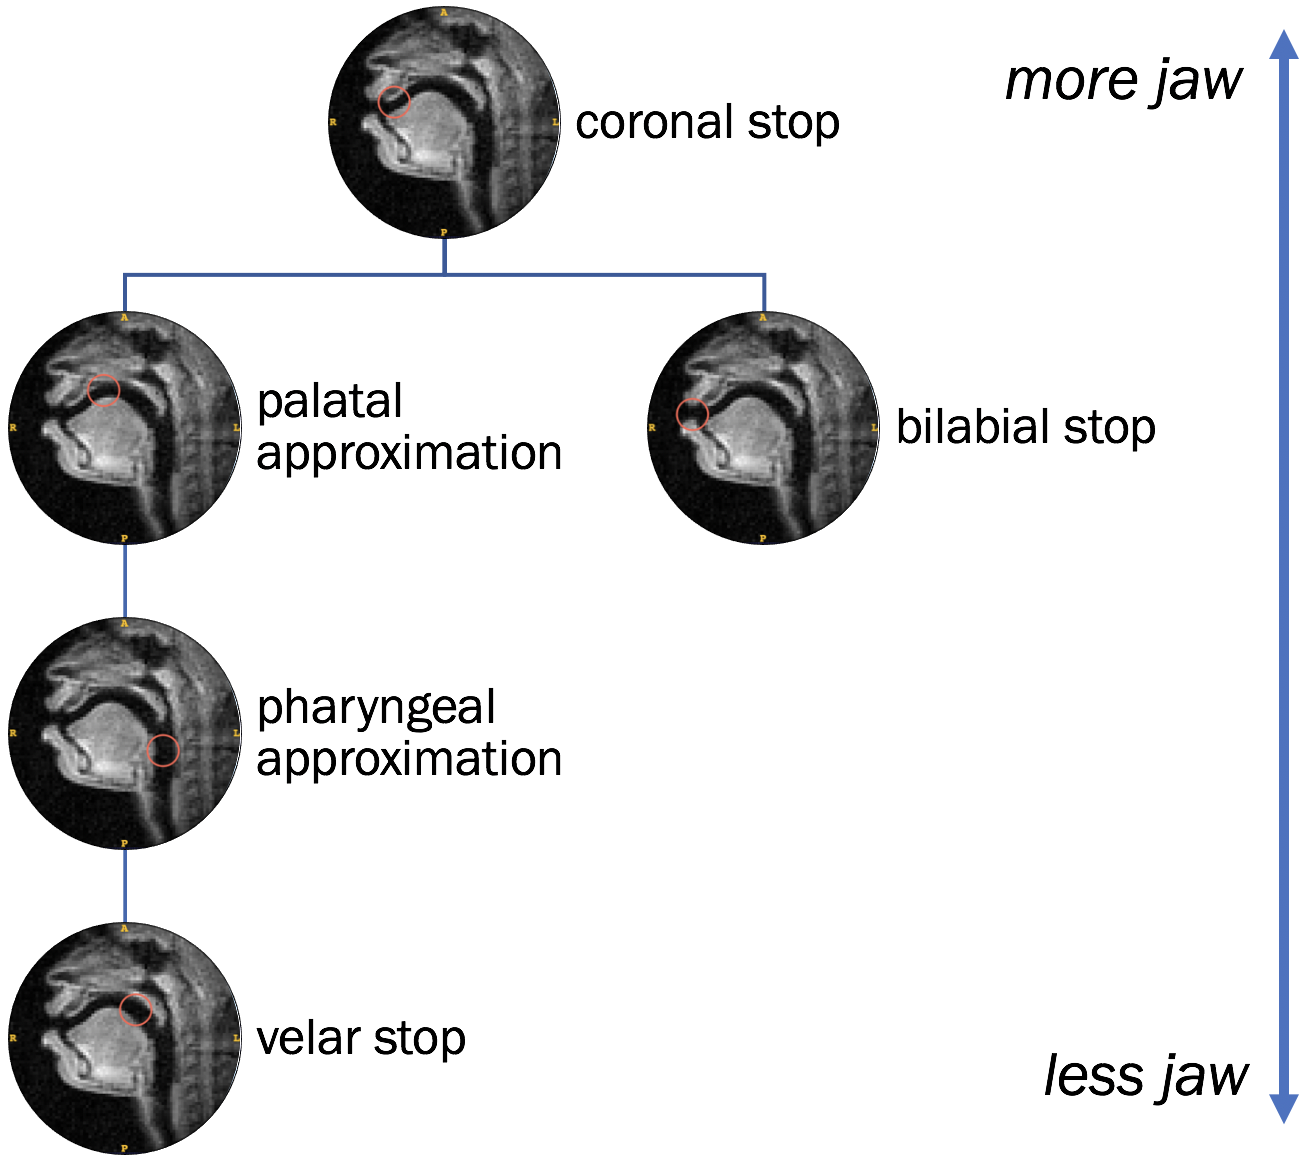
\includegraphics[width=\linewidth]{task_spec_summary.png}

\caption{(color online) Synergies differ in terms of inter-articulator coordination depending on the constriction task. Constriction tasks are ordered from top to bottom in terms of jaw usage. Vertical lines indicate a statistically significant contrast. Compare with numeric results in Table~\ref{tab:stat_results}.}
\label{fig:task_spec_summary}
\end{figure}




The sample distribution of the articulator synergy biomarker for the velar stop had small dispersion about a distinct peak at \SI{10}{\percent} 
%
(median: \SI{12}{\percent}, 
inter-quartile range: \SIrange{7.3}{24}{\percent}; see histograms in Fig.~\ref{fig:histograms}).
%
The sample distribution of the articulator synergy biomarker for the coronal stop had a distinct peak at \SI{60}{\percent}
%
(median: \SI{56}{\percent}, 
inter-quartile range: \SIrange{44}{64}{\percent}; see histograms in Fig.~\ref{fig:histograms}).
%
The distinctly peaked sample distributions of the articulator synergy biomarkers for the coronal stop and velar stop likely contributed to the statistically significant bilabial stop-velar stop, coronal stop-palatal approximation, coronal stop-velar stop, palatal approximation-velar stop, palatal approximation-pharyngeal approximation, velar stop-pharyngeal approximation, and coronal stop-pharyngeal approximation contrasts.



In order to determine whether the results reported above depended on the choice of a particular number of jaw, tongue, and lip factors or on the choice of a particular neighborhood size for the forward kinematic map estimator, we repeated the statistical analysis with different parameter values (number of jaw factors: 1, 2, 3; number of tongue factors: 4, 6, 8; number of lip factors: 2, 3; neighborhood size: \SIrange{20}{90}{\percent} in \SI{10}{\percent} steps).
%
The articulator synergy biomarker was greater for the coronal stop than for the 
%
bilabial stop in 96/96 cases 
(\SI{100}{\percent}), 
%
palatal approximation in 32/96 cases
(\SI{33}{\percent}), 
velar stop in 88/96 cases 
(\SI{92}{\percent}), 
and pharyngeal approximation in 83/96 cases
(\SI{86}{\percent}).
%
The articulator synergy biomarker was greater for the palatal approximation than for the 
%
velar stop in 71/96 cases
(\SI{74}{\percent})
and pharyngeal approximation in 65/96 cases
(\SI{68}{\percent}).
%
The articulator synergy biomarker was greater for the pharyngeal approximation than for the 
%
velar stop in 25/96 cases 
(\SI{26}{\percent}).
%
Overall, these results support the inference that the jaw contributed significantly more to the coronal stop than to the bilabial stop and velar stop,
%
and that the jaw contributed significantly more to the palatal approximation than to the velar stop.
%
However, the coronal stop-palatal approximation, coronal stop-pharyngeal approximation, palatal approximation-pharyngeal approximation, and velar stop-pharyngeal approximation contrasts should be interpreted with caution, since the effect size is smaller than for the more robust effects and the significance of these contrasts depends on parameterization.



In sum, the present study shows that the jaw contributes 
least to the velar stop for \textipa{[k]},
more to pharyngeal approximation for \textipa{[A]}, 
still more to palatal approximation for \textipa{[i]},
and most to the coronal stop for \textipa{[t]}.
Additionally, the jaw contributes more to the coronal stop for \textipa{[t]} than to the bilabial stop for \textipa{[p]} (see Fig.~\ref{fig:task_spec_summary}).








\section{Inter- and intra-participant variability}
\label{sec:patterns}





Section~\ref{sec:taskspec} shows an effect of constriction task on the articulator synergy biomarker values. 
%
This section investigates inter- and intra-participant variability in this effect.
%
Inter-participant variability is evaluated by testing the significance of by-participant random slopes for constriction task.
%
The linear mixed effects model of Section~\ref{sec:taskspec} (cf. Equation~\ref{eq:lmm}) is compared to a reduced model that does not have by-participant random slopes for constriction task.
%
The likelihood ratio test indicates that the by-participant random slopes for constriction task are a significant source of variance ($\chi^2(14)= 560; p = \ensuremath{1.7\times 10^{-109}}$).
%
This indicates variability by participant in the effect for constriction task.
%
By-participant variability in the effect for constriction task is further characterized by determining whether individual participants display similar effects for constriction task (i.e., same pattern of average values) and similar variances across constriction tasks.
%
For each participant, the Mann-Whitney U Test identifies all pairs of constriction tasks that differ in average biomarker value,
and the Fligner-Killeen Test identifies all pairs of constriction tasks that differ in biomarker variance (see Fig.~\ref{fig:consistency}).
%
The study performed (number of participants) $\times$ ((number of constriction tasks)\textsuperscript{2} - (number of constriction tasks))/2 $=$ \num{80} Mann-Whitney U Tests and the same number of Fligner-Killeen tests for a total of \num{160} statistical tests. 
%
Statistical tests are considered significant at the Bonferroni-corrected significance level $\alpha = 0.05/160$.


The results of the Mann-Whitney Tests demonstrate that the pattern of average values across constriction tasks is consistent with the effect for constriction task discovered by the linear mixed effects model (coronal stop $>$ palatal approximation $>$ pharyngeal approximation $>$ velar stop; and coronal stop $>$ bilabial stop; cf. Section~\ref{sec:taskspec}) with three exceptions: velar stop-pharyngeal approximation constrast of participant m1; palatal approximation-velar stop and palatal approximation-pharyngeal approximation constrasts of m4.
Although the participants individually display consistent patterns of average values, the dispersion of the data is large and the sample size within each participant is small.
For this reason, the Mann-Whitney U Test does not reject all the null hypotheses.

The results of the Fligner-Killeen Tests demonstrate that participants can display high biomarker variance for some constriction tasks but low variance at others. However, fewer Fligner-Killeen Tests reject the null hypothesis than do the Mann-Whitney U Tests. This indicates that fewer variances differ by constriction task than do the average values.

\begin{figure*}

\includegraphics[width=\linewidth]{ConsistencyFigure.pdf}

\caption{(color online) Sample distribution of the articulator synergy biomarker (y-axis) by participant (panel) and by constriction task (color, x-axis). Kernel density estimate (shaded) and \SI{95}{\percent} confidence interval for the mean (whiskers) provided for each distribution.
%
Brackets below each panel indicate pairs of constriction tasks that significantly differ in average value (Mann-Whitney Test) or variance (Fligner-Killeen Test). $p$-values corrected for multiple comparisons with the Bonferroni method. Adjusted $p$-values used to determine significance.}
\label{fig:consistency}
\end{figure*}






\section{Discussion}
\label{sec:discussion}

\subsection{Task specificity of articulator synergies}

The present study shows that the jaw contributes 
least to the velar stop for \textipa{[k]},
more to pharyngeal approximation for \textipa{[A]}, 
still more to palatal approximation for \textipa{[i]},
and most to the coronal stop for \textipa{[t]}.
Additionally, the jaw contributes more to the coronal stop for \textipa{[t]} than to the bilabial stop for \textipa{[p]}.
%
This supports the hypothesis that different articulator synergies have different patterns of inter-articulator coordination.


The effect of constriction type on the articulator synergy biomarker demonstrates that inter-articulator coordination differs depending on the constriction task. Jaw usage varies by place of articulation (i.e., constriction location), by active articulator (i.e., end-effector), and by manner of articulation (i.e., target constriction degree)~\cite{vatikiotis1995analysis}. Both of these sources of variance presumably combine to produce the effect of constriction type reported in this paper. This introduces a confound in interpreting the effect for constriction task, and thus is a limitation of the present study. Future research should focus on how place and manner of articulation interact to determine articulator synergy biomarker values.


If synergies organize the articulators on a temporary basis for achieving motor goals such as vocal tract constrictions, as proposed in theories of motor control~\citep{turvey1977preliminaries, saltzman1987skilled}, theories of phonological organization~\citep{browman1986towards, browman1989articulatory}, and robotic systems~\citep{herbort2010sure}, then the pattern of inter-articulator coordination varies over time as the vocal tract deploys different synergies. 
%
The articulator synergy biomarker provides the means to characterize this time-varying pattern of inter-articulator coordination in terms of the percent contribution of each articulator to changing the constriction task variable at the synergy's place of articulation. 
%
This complements the finding that articulator synergies are task-dependent in terms of inter-articulator coupling~\citep{lancia2018coupling}, inter-articulator correlation~\citep{jackson2009statistical}, and response to mechanical perturbation of articulator positions~\citep{kelso1984functionally}.


\subsection{Technical performance}

The proliferation of vocal tract imaging databases~\citep{narayanan2014real,sorensen2017database} and the increasingly complex computational methods for studying the morphological~\citep{lammert2013morphological} and functional~\citep{dawson2016methods} complexities captured therein underscore the importance of evaluating the technical performance of quantitative imaging biomarkers of speech. 
%
The articulator synergy biomarker does not have systematic bias. However, precision is weak or poor at the coronal stop, velar stop, and pharyngeal approximation. 
%
Since the intra-class correlation coefficient is the ratio of inter-participant variability to total
variability, which is the sum of intra- and inter-participant variability (cf. Equation~\ref{eq:icc}), low precision may be due to large intra-participant variance, small inter-participant variance, or some combination of the two. 
%
For the velar stop, low precision is due to small inter-participant variance (cf. Fig.~\ref{fig:histograms}). 
%
For the coronal stop and pharyngeal approximation, low precision is due to large intra-participant variance.
%
Intra-participant variance is unavoidable in voluntary movement due to short-term physiological variability that arises from the way the brain regulates noise in the motor system~\citep{harris1998signal,van2009motor,wu2014temporal}. 
%
Although we do not discount other technical sources of variance such as MRI operator variability and image analysis variability, here we emphasize short-term physiological variability as the fundamental obstacle to achieving high precision in biomarkers of voluntary movement.





\subsection{Parametric estimation for Task Dynamics}



The forward kinematics relates articulator movements to the changes in constriction task variables that these movements produce. 
%
In the Task Dynamics model of speech production~\citep{saltzman1989dynamical}, the forward kinematics is specified by the forward kinematic map and its jacobian matrix. 
%
The study estimated these parameters from real-time MR images of speech production and evaluated the estimator by cross-validation. Error was well below the spatial resolution of the scanner.



The inverse kinematics relates changes in constriction task variables to the articulator movements that produce them. 
%
In the Task Dynamics model of speech production~\citep{saltzman1989dynamical}, the percent contribution of each articulator in a synergy is determined by assigning weights to the articulators. 
%
In contrast to studies that manually assigned weights to the articulators based on theoretical considerations~\citep[for example, see][for an assignment of weights based on articulator mass]{simko2010embodied}, the present study is the first to obtain a quantitative readout of these weights from speech production data. 
%
Analysis of synthetic data in Section~\ref{subsec:bias} suggested that the articulator synergy biomarker is a monotonic function of the jaw weight parameter (Fig.~\ref{fig:valfig}, panel a).
%
The function will depend on the number of articulator degrees of freedom, the coordinate system for the articulator degrees of freedom, the constriction task, and the weights of other articulators. Further work is necessary to characterize these sources of variance, but the present study suggests that the articulator synergy biomarker can be mapped to articulator weights, and thus that jaw weight parameters can be estimated from real-time MR images of speech production.




\subsection{Decomposing the tongue into multiple articulators}

For coronal stop \textipa{[t]}, palatal approximation \textipa{[i]}, velar stop \textipa{[k]}, and pharyngeal approximation \textipa{[A]} constriction tasks,
the articulator synergy indicates the relative contribution of the jaw and tongue.
%
For example, a biomarker value of \SI{60}{\percent} indicates a jaw contribution of  \SI{60}{\percent}. The remaining \SI{40}{\percent} is understood to come from the tongue.
%
The present study considers the contribution of the tongue in aggregate and does not decompose its contribution into subparts such as tongue body and tongue tip.
%
An extension of the articulator synergy biomarker would be to consider not simply a binary distinction between jaw and tongue, but an ternary distinction among jaw, tongue body, and tongue tip or even a quaternary distinction among jaw, tongue root, tongue dorsum, and tongue tip.
%
This section provides a preliminary indication of how this is possible within the framework presented in the present study.



The method by which Section~\ref{sec:gfa} obtained jaw factors offers a recipe for obtaining factors that are associated with the motion of a subset of data-points. 
First, we obtain the jaw factors (Fig.~\ref{fig:extensionsfigure}, Panel B) as in Section~\ref{sec:gfa}.
The null space of the transposed jaw factors captures the part of tongue and lip motion that is independent of jaw motion. 

Second, we project the data matrix on the null space of the transposed jaw factors as in Section~\ref{sec:gfa}. This is the contour motion that is independent of the jaw.
Rather than subject the whole tongue contour to principal component analysis as in Section~\ref{sec:gfa}, we perform principal component analysis only on the tongue body contour vertices.
The tongue body factors (Fig.~\ref{fig:extensionsfigure}, Panels C and D) are the vectors of covariances between the z-scored tongue body principal component scores and the tongue body and tongue tip contour vertices.
The null space of the transposed set of jaw and tongue body factors captures the part of tongue tip motion that is independent of jaw and tongue body motion.

Third, we project the data matrix on the null space of the transposed jaw and tongue body factors. This is the contour motion that is independent of the jaw and tongue body.
We perform principal component analysis on the tongue tip contour vertices.
The tongue tip factors (Fig.~\ref{fig:extensionsfigure}, Panel E) are the vectors of covariances between the z-scored tongue tip principal component scores and the tongue tip contour vertices.
The null space of the transposed set of jaw, tongue body, and tongue tip factors captures residual variance that is independent of jaw, tongue body, and tongue tip motion.

Whereas Section~\ref{sec:gfa} extracts all tongue factors from the null space of the transposed jaw factors, the procedure described above extracts tongue body factors from the null space of the transposed jaw factors and then extracts tongue tip factors from the null space of the transposed jaw and tongue body factors.
This procedure offers a systematic way to decompose the tongue into subparts that form a kinematic chain~\cite{craig2005introduction}. Future work that pursues this approach will provide greater detail in the analysis of jaw-tongue coordination in synergies.

\begin{figure}

\includegraphics[width=\linewidth]{ExtensionsFigure.pdf}

\caption{(color online) {\bf a.} Operational definition of jaw, tongue body, and tongue tip contours.
{\bf b-e.} Mean vocal tract contour (black) with jaw, tongue body ($\times$\num{2}), and tongue tip factors overlaid (red contour: +\num{2} S.D.; blue: -\num{2} S.D.).}
\label{fig:extensionsfigure}
\end{figure}





\subsection{Forward kinematics and the nervous system}

The nervous system has an internal model of the forward kinematics~\citep{shadmehr2010error, guenther2016neural}. This model encodes the expected result of motor commands in terms of expected sensory consequences (proprioceptive and auditory consequences in the case of speech). 
%
Both the forward kinematics of the vocal tract and the nervous system's internal model of the forward kinematics are important components of a computational model of motor control  (for a theoretical model of speech motor control that cleanly distinguishes these components, see \citealt{Ramanarayanan+2016}; cf. ``forward kinematics'' and ``model of forward kinematics'' blocks; see also \citealt{houde2011speech,todorov2002optimal}). Although the present study estimates the forward kinematics, it does not characterize the nervous system's internal model of the forward kinematics. While both relate the articulator degrees of freedom to task variables, the coordinate system that represents the articulator degrees of freedom in the nervous system may differ from the coordinate system of the present study. That is, the nervous system may represent the articulator degrees of freedom differently than with jaw, tongue, and lip factors. If the coordinate system for the nervous control of vocal tract movement were known, insight into motor variability, motor equivalence, and redundancy could be gleaned from analysis of the forward kinematic map using the uncontrolled manifold approach~\cite{scholz1999uncontrolled}. However, the results of such studies are inconclusive without knowledge of the coordinate system used in the nervous system~\cite{sternad2010coordinate}. Knowledge of the coordinate system could potentially be obtained through detailed modeling of the innervation of head and neck muscles. Indeed, physiological knowledge guides the choice of coordinate system for analysis of the uncontrolled manifold in human upper limb movement (cf. argument of~\citealt{scholz2014use}, \S~7.1, Point~3).
Biomechanical models offer tools for investigating the coordinate system available to the nervous system for producing vocal tract movements~\cite{lloyd2012artisynth}. \citet{Szabados+2016} used a biomechanical model to investigate motor equivalence using the uncontrolled manifold approach. Future work should investigate whether MRI can be used to model the nervous system's internal model of the forward kinematics of the vocal tract. 






\section{Conclusions}
\label{sec:conclusions}

The present study shows that the jaw contributes 
least to the velar stop for \textipa{[k]},
more to pharyngeal approximation for \textipa{[A]}, 
still more to palatal approximation for \textipa{[i]},
and most to the coronal stop for \textipa{[t]}.
Additionally, the jaw contributes more to the coronal stop for \textipa{[t]} than to the bilabial stop for \textipa{[p]}.
%
This supports the idea that synergies organize the articulators on a temporary basis for achieving motor goals such as vocal tract constrictions, and that the pattern of inter-articulator coordination varies over time as the vocal tract deploys different synergies. 




The following are four potential threads of research that build on the results of the present study.
%
First, the present study estimated parameters of vocal tract \textit{kinematics}, not parameters of vocal tract \textit{dynamics}. That is, the parameters have to do with motion, not with the forces that produce the motion. In the Task Dynamics model of speech production, dynamical parameters include gestural parameters (e.g., stiffness, damping, mass) and parameters of inter-gestural coordination (e.g., coupling, blending). Future studies may attempt to estimate these parameters from MRI.
%
Second, the present study showed that the articulator synergy biomarker varied by constriction task. Future studies may evaluate whether the articulator synergy biomarker depends on linguistic context (e.g., phonetic, lexical, syntactic), speech conditions (e.g., speech in noise vs. clean speech, variable speech rate), sociolinguistic factors, sex, anatomy, and age, especially during childhood development.
%
Third, while the present study focused on jaw-tongue and jaw-lip synergies, the proposed method could be used to study other synergies, such as those between the dorsum and tip of the tongue or between the tongue and velum. Future research studies should investigate these synergies.
%
Fourth, a forward kinematic map from articulators to acoustic formant frequencies is used by the Directions into Velocities of Articulators (DIVA) model of speech production~\cite{guenther1995speech}. By using real-time MRI with simultaneously recorded speech audio, the proposed framework could be extended to estimate this forward kinematic map from data.




\section{Reproducibility and replication}

The scripts required to reproduce the present study are available at \url{https://github.com/TannerSorensen/task_spec_synergies}.
%
The MRI data-set is available at \url{http://sail.usc.edu/span/test-retest/} for free use by the research community~\citep[see][]{toger2017test}.
%
A replication of the present study was performed using the USC Speech and Vocal Tract Morphology MRI Database~\citep{sorensen2017database} and is available as supplementary material.\footnote{The results of the replication study are available at [URL will be inserted by AIP].}

\section{Acknowledgments} 

The authors acknowledge funding through NIH grant R01DC007124, NIH grant T32DC009975, and NSF grant 1514544. The content of this paper is solely the responsibility of the authors and does not necessarily represent the official views of the NIH or NSF.

\bibliography{mybib.bib}

\end{document}
